\documentclass[11pt]{article}
\usepackage[review]{acl}
\usepackage{times}
\usepackage{latexsym}
\usepackage[T1]{fontenc}
\usepackage[utf8]{inputenc}
\usepackage{microtype}
\usepackage{graphicx}
\usepackage{booktabs}
\usepackage{amsmath}
\usepackage{amssymb}
\usepackage{amsthm}

\newtheorem{proposition}{Proposition}
\newtheorem{remark}{Remark}

\title{What Is a Persona Worth?\\
Pricing LLM Human Simulation in Human Answers}

\author{Anonymous ARR submission}

\begin{document}
\maketitle

\begin{abstract}
An LLM persona is supposed to stand in for a person. We make that claim
measurable by pricing it in the only currency a practitioner actually spends:
questions asked of a real human. The \emph{answer-equivalent} $m^{*}$ of a
simulator is the number of a respondent's own answers a conditional model needs
before it predicts that respondent's remaining answers as well as the simulator
does. It is defined against a strictly proper ordinal score, it is selected
entirely on held-out respondents, and it does not presuppose its own answer:
$m^{*}{=}40$ would be strong evidence that persona prompting substitutes for a
questionnaire. We first show why a proper score is required at all --- under the
answer-similarity metric these systems are validated with, a simulator that
reproduces the target population's response distribution \emph{exactly} can never
beat a constant vector, and is strictly beaten on all $480$ cluster--item
combinations of $410{,}168$ IPIP-NEO-120 respondents. We then price $72$
(model $\times$ instrument $\times$ panel) cells spanning four inventories and
fifteen open models, including a held-out family of $180$ IPIP-NEO-300 items the
same respondents answered. The answer-equivalent is stable across disjoint
respondent panels (Spearman $\rho{=}0.78$, $p{<}10^{-6}$) and orders models
consistently: the strongest persona we measure is worth $5.38$ of $120$ answers
on the unseen item family and $3.07$ of $60$ on the short form, the weakest
exactly $0$. What separates them is not accuracy but the sharpness of each model's
person-conditional belief: controlling for accuracy, belief entropy predicts the
price at $\rho{=}-0.52$, and the share of person-specific deviation surviving
calibration at $\rho{=}+0.66$, and how the observations are presented: a $30$-line trait profile is
worth almost five times the raw transcript of the same $120$ answers. Finally we
bound the result: across $160$ cells and three combination families --- convex,
linear, and gradient-boosted --- adding a persona to a conditional model of the
respondent's own observed answers yields a selected weight of $0$ in $127$ cells
and never above $0.05$; of $426$ tests one survives multiplicity control, and it
reverses sign on its own disjoint panel. A persona carries a small,
real, model-scaling amount of personal information that a handful of real answers
renders redundant. We release the instrument, the code and all per-cell results.
\end{abstract}

\section{Introduction}
\label{sec:intro}

A practitioner deciding whether to simulate respondents instead of recruiting
them is asking a quantitative question: how many real answers is the simulator
worth? The literature does not answer it. Simulators are reported as
correlations, agreement scores, or wins over a baseline, none of which convert
into the resource the decision actually trades against --- questions put to a
real person.

We supply that conversion. The \emph{answer-equivalent} $m^{*}$ of a simulator is
the number of a respondent's own answers a conditional model needs before it
predicts that respondent's remaining answers as well as the simulator does.

Two properties make it usable. First, it is anchored to a strictly proper score,
which is not optional here: the answer-similarity metric these systems are
validated with has a degenerate optimum, and under it a simulator that reproduces
the target population's response distribution \emph{exactly} is dominated by a
constant vector (\S\ref{sec:theory}). A price quoted in an improper currency is
not a price. Second, it does not presuppose its answer. Every quantity is
selected on held-out respondents, and $m^{*}{=}40$ would be strong evidence that
persona prompting substitutes for a questionnaire. That symmetry is what makes
the number we do measure worth reporting.

Our contributions are:

\begin{enumerate}\itemsep2pt
\item \textbf{The answer-equivalent} (\S\ref{sec:equiv}): an instrument that
prices any respondent simulator in units of the respondent's own answers, under a
strictly proper ordinal score, with every hyperparameter selected on held-out
respondents and the baseline's capacity retuned at each budget.
\item \textbf{Why a proper score is required} (\S\ref{sec:theory}): under
answer-similarity, an exactly faithful simulator is dominated by the best
constant predictor --- strictly so on all $480$ cluster--item combinations we
measure. The penalty is the excess of the Gini mean difference over the mean
absolute deviation about the median, divided by the scale range.
\item \textbf{A price, at scale} (\S\ref{sec:price}): $89$ cells over five
inventories and fifteen open models, including transfer to $180$ unseen items the
same people answered. $m^{*}$ replicates across disjoint respondent panels
($\rho{=}0.78$) and reaches $5.38$ answers where human labels are scarcest.
\item \textbf{A mechanism} (\S\ref{sec:why}): $m^{*}$ is governed by the
share of a model's person-specific deviation that survives population
calibration, not by its accuracy.
\item \textbf{A boundary} (\S\ref{sec:boundary}): across $160$ cells and three
combination families, a persona adds no predictive information beyond a
conditional model of the respondent's own observed answers; the selected
combination weight is $0$ in $127$ cells and never exceeds $0.05$.
\end{enumerate}

\section{Setting}
\label{sec:setting}

\paragraph{Task.} A population of respondents is partitioned into $K$ personality
clusters by $k$-means over the 30 IPIP-NEO facet scores. For each cluster a
natural-language description is used to condition an LLM, which then answers the
120 IPIP-NEO items on a 1--5 Likert scale. Prompt wording is optimised by an
evolutionary search whose fitness is answer agreement with held-out human
members of the cluster.

Two regimes appear here and are not interchangeable. The \emph{cluster} regime
conditions on the centroid alone, giving every member one prompt; it is what
Prop.~\ref{prop:main} and the $7.75$-point penalty address. The
\emph{individual} regime, used by the released prompt builder and by
\S\ref{sec:mechanism}, inserts each respondent's own scores as intensity
modifiers. By Remark~\ref{rem:conditional} one constant is optimal in the
first and a per-respondent conditional median in the second; we name the
regime wherever a result depends on it.

\paragraph{The metric.} A simulated answer vector $x$ is scored against a human
answer vector $y$ by
\begin{equation}
S(x,y) \;=\; \frac{1}{J}\sum_{j=1}^{J}\Big(1 - \tfrac{|x_j - y_j|}{4}\Big),
\label{eq:metric}
\end{equation}
with $J{=}120$ and the divisor $4$ the scale range. Cell scores average
$S$ over the held-out respondents. Equation~\eqref{eq:metric}, or a monotone
transform of it, is the objective the search optimises and the number reported.

\section{A constant is optimal under $S$}
\label{sec:theory}

Fix a cluster and an item $j$, and let $P_j$ be the cluster's response
distribution over $\{1,\dots,5\}$. Write $Y\sim P_j$ for a randomly drawn human
respondent.

\begin{proposition}
\label{prop:main}
Let $m_j$ be a median of $P_j$, let
$\mathrm{MAD}_j = \mathbb{E}_Y|m_j - Y|$ and let
$\mathrm{GMD}_j = \mathbb{E}_{X,Y}|X-Y|$ for $X \sim P_j$ independent of $Y$
(the Gini mean difference). Then
\begin{enumerate}\itemsep0pt
\item[(a)] the best constant predictor attains expected score
$1 - \mathrm{MAD}_j/4$;
\item[(b)] a \emph{faithful} simulator, i.e.\ one whose output is distributed as
$P_j$, attains expected score $1 - \mathrm{GMD}_j/4$;
\item[(c)] $\mathrm{GMD}_j \ge \mathrm{MAD}_j$, with equality iff $X$ lies
almost surely in the median set of $P_j$.
\end{enumerate}
Hence the constant is at least as good as the faithful simulator, and strictly
better unless $P_j$ places all its mass on medians.
\end{proposition}

\begin{remark}[Where this applies]
\label{rem:conditional}
Proposition~\ref{prop:main} is unconditional; the audited systems condition on
something. Let $C$ be everything the simulator observes, its draw independent of
the response given $C$. Under \eqref{eq:metric} an optimal simulator emits a
\emph{conditional} median $m_j(C)$, so one constant stays optimal exactly when
the conditional median sets share a value almost surely, item by item.
Cluster-only conditioning thus admits a cluster-specific constant optimum;
individually informative conditioning can make different deterministic answers
optimal, so the constant need not win. A deterministic conditional median is
always optimal and a randomised predictor ties exactly when its support lies in
that median set, so absolute error never \emph{uniquely} rewards faithful
conditional sampling; richer conditioning moves which prediction is rewarded.
\end{remark}

\begin{proof}
(a) and (b) are immediate from \eqref{eq:metric}. For (c),
\begin{align*}
\mathrm{GMD}_j &= \mathbb{E}_X\big[\mathbb{E}_Y|X-Y|\big]\\
&\ge \mathbb{E}_X\big[\textstyle\min_{c}\mathbb{E}_Y|c-Y|\big]\\
&= \mathbb{E}_Y|m_j-Y| \;=\; \mathrm{MAD}_j,
\end{align*}
since the median minimises expected absolute deviation. Equality requires $X$
to attain that minimum almost surely, i.e.\ to lie in the median set of $P_j$.
This is weaker than degeneracy: a balanced two-point law
$P(Y{=}1)=P(Y{=}5)=\tfrac12$ has $\mathrm{GMD}=\mathrm{MAD}=2$, so the bound is
tight there despite large variance. On the IPIP items it is strict throughout
(Table~\ref{tab:proposition}).
\end{proof}

The consequence is not a technicality. Under $S$ the behaviour we want ---
reproducing the population's response distribution --- is penalised relative to
one fixed vector, so the optimum is degenerate in exactly the variance that
carries a profile. Whether an optimiser is driven there is empirical and not
uniform: $S_0$ ships a near-worst model from a heterogeneous pool
(App.~\ref{app:rules}), yet prompt search under it improves proper scores too
(App.~\ref{app:whenbites}).

\subsection{The metric is CRPS with its dispersion term deleted}
\label{sec:crps}

Proposition~\ref{prop:main} is not an accident of Likert data. The continuous
ranked probability score for a predictive distribution $F$ and outcome $y$ is
\[
\mathrm{CRPS}(F,y)=\mathbb{E}_F|X-y|-\tfrac{1}{2}\,\mathbb{E}_F|X-X'| ,
\]
and it is \emph{strictly proper}: uniquely optimised by $F=P$. Equation
\eqref{eq:metric} is its first term alone. Deleting the second is exactly what
makes a constant optimal.

This yields the natural repair. Define
\begin{equation}
S_\lambda \;=\; 1-\big[\,\mathbb{E}|X-y|-\lambda\,\mathbb{E}|X-X'|\,\big]/4 ,
\label{eq:slambda}
\end{equation}
$\lambda{=}0$ is the audited metric --- improper, constant-optimal. $\lambda{=}1/2$
is CRPS --- strictly proper, truth-optimal. $\lambda{>}1/2$ is improper in the
opposite direction. $\lambda{=}1/2$ is the unique proper choice, not a tunable
hyperparameter.

Sweeping $\lambda$ over the same 20 cells (Table~\ref{tab:lambda}) shows the
repair works and what it costs the simulator. At $\lambda{=}1/2$ the human
ceiling ($0.859$) rises decisively above the constant floor ($0.796$): the
ordering that \S\ref{sec:ceiling} shows is inverted under the audited metric is
\emph{correct} under the proper one. Humans overtake the constant at
$\lambda^\star{=}0.30$, comfortably below the proper coefficient. The model needs
$\lambda^\star{=}0.75$ (median grid crossover; $0.757$ on the aggregate
curve) --- a rule that over-rewards dispersion --- and beats the
constant in only $2$ of $20$ cells at the proper $\lambda{=}1/2$, though it does
overtake in most cells once $\lambda$ reaches $1$, where the reward for
dispersion is twice proper. So the simulator's
failure is not an artefact of a bad metric: it survives the correct one.

so larger is better. Scores in the appendices are reported as the
corresponding \emph{loss} $L_{1/2}=1-S_{1/2}$, the normalised CRPS, where
smaller is better; we use the loss wherever a table compares errors and mark
the direction in each caption.

\begin{table}[t]\centering\footnotesize
\setlength{\tabcolsep}{4pt}
\begin{tabular}{lccc}
\toprule
$\lambda$ & Model & Constant & Human\\
\midrule
$0$ \;(audited) & 0.726 & \textbf{0.796} & 0.720\\
$0.25$ & 0.749 & \textbf{0.796} & 0.789\\
$0.5$ \;(CRPS, proper) & 0.772 & 0.796 & \textbf{0.859}\\
$0.75$ & 0.795 & 0.796 & \textbf{0.929}\\
$1.0$ & 0.819 & 0.796 & \textbf{0.998}\\
\bottomrule
\end{tabular}
\caption{The $S_\lambda$ family of \eqref{eq:slambda}, averaged over 20 cells, all
values on the corrected orientation. A constant wins at the audited
$\lambda{=}0$; at the proper $\lambda{=}1/2$ a real cluster member wins, as it
must. All-pairs scores, slightly below the paired ones of \S\ref{sec:audit};
the ordering is the same under either.}
\label{tab:lambda}
\end{table}

Table~\ref{tab:proposition} evaluates the bound on the real data: the structural
penalty against a faithful simulator averages \textbf{7.75 points}, and
$\mathrm{GMD}_j \ge \mathrm{MAD}_j$ holds on $120/120$ items in all four clusters.

\begin{table}[t]\centering\footnotesize
\setlength{\tabcolsep}{3.5pt}
\begin{tabular}{lccccc}
\toprule
Clu. & $n$ & MAD & GMD & $S_{\mathrm{const}}$ & $S_{\mathrm{faith}}$\\
\midrule
0 & 107,174 & 0.804 & 1.107 & 0.7990 & 0.7232\\
1 & 108,880 & 0.723 & 1.008 & 0.8192 & 0.7480\\
2 & 108,867 & 0.809 & 1.128 & 0.7978 & 0.7181\\
3 & 85,247 & 0.871 & 1.204 & 0.7822 & 0.6990\\
\midrule
Mean & & 0.802 & 1.112 & \textbf{0.7996} & 0.7221\\
\bottomrule
\end{tabular}
\caption{Proposition~\ref{prop:main} on $410{,}168$ IPIP-NEO-120 respondents.
$S$(const) is the best constant predictor; $S$(faithful) is a simulator that
reproduces the cluster response distribution exactly. The faithful simulator is
worse in every cluster.}
\label{tab:proposition}
\end{table}

\section{Empirical audit}
\label{sec:audit}

\paragraph{Setup.} We re-score an existing cluster-level digital-twin system on
its own artefacts: the same $410{,}168$-respondent IPIP-NEO-120 corpus, the same
$k{=}4$ clusters, and the exact train/test respondent IDs it recorded, for five
LLMs (GigaChat3-10B, GPT-4.1-mini, GPT-4.1-nano, Grok-4.1-fast, Qwen3-235B)
$\times$ four clusters. We add no LLM calls: model answers are read from the
released run artefacts. Baselines are fitted on the recorded train IDs and scored
on the recorded test IDs.

\paragraph{Baselines.} \textit{Cluster mean}: the per-item rounded mean of the
cluster's training respondents, one constant vector. \textit{Cluster majority}:
the per-item mode. \textit{Global mean}: the per-item grand mean over all
respondents, ignoring clusters. \textit{Empirical sample}: sample each item
independently from the cluster's training response distribution. \textit{Real
human}: copy the answer vector of a randomly chosen training respondent from the
same cluster.

\paragraph{Result.} Table~\ref{tab:headtohead} reports $S$. The evolutionary
persona averages $0.660$ as released and $0.739$ after the orientation
correction of \S\ref{sec:orientation}; the constant cluster mean averages
$0.796$. The LLM loses in $20$ of $20$ cells under either orientation, by $13.6$
and $5.8$ points respectively. What survives correction is \emph{matched-cell}
dominance: the model loses to its own cluster's constant in every cell, while its
best cell ($0.807$) now exceeds the weakest constant elsewhere ($0.779$), so the
comparison only holds within a cluster. A per-item global mean --- which never
looks at the cluster at all --- scores $0.774$, still above the persona's
corrected $0.739$.

\begin{table*}[t]\centering\small
\begin{tabular}{lccccc}
\toprule
Model & \multicolumn{4}{c}{Cluster} & Mean\\
\cmidrule(lr){2-5}
 & 0 & 1 & 2 & 3 & \\
\midrule
GPT-4.1-mini & 0.657 & 0.638 & 0.710 & 0.652 & 0.664\\
GPT-4.1-nano & 0.673 & 0.678 & 0.697 & 0.670 & 0.679\\
GigaChat3-10B & 0.711 & 0.691 & 0.737 & 0.672 & 0.703\\
Grok-4.1-fast & 0.598 & 0.583 & 0.659 & 0.614 & 0.613\\
Qwen3-235B & 0.634 & 0.615 & 0.677 & 0.642 & 0.642\\
\midrule
\textit{Cluster mean} (constant) & \textbf{0.794} & \textbf{0.827} & \textbf{0.785} & \textbf{0.779} & \textbf{0.796}\\
\textit{Real human, same cluster} & 0.720 & 0.747 & 0.715 & 0.704 & 0.721\\
\bottomrule
\end{tabular}
\caption{Answer similarity $S$ on the original system's own test IDs, in the
\emph{original} orientation; correction adds $0.079$ on average and preserves
all $20$ matched constant wins, though it does reorder the models. The constant
(bold) beats every LLM in every cell; a real human scores below it.}
\label{tab:headtohead}
\end{table*}

\section{Does conditioning on the right cluster matter?}
\label{sec:permutation}

Correct cluster assignment does help, and by far too little to matter: the
permuted-cluster control is worse than the correct one, but both are worse
than a constant. Appendix~\ref{app:permutation} gives the per-cell numbers.
The individual-level version of this control --- correct respondent versus
shuffled respondent --- is what \S\ref{sec:equiv} prices, and it is the
version that bears on whether a persona simulates a \emph{person}.

\section{An orientation defect, and what survives it}
\label{sec:orientation}

The released benchmark scores raw model self-reports against
reverse-recoded human answers on $55$ of $120$ items. Correcting it lifts
the correlation of per-item means from $+0.09$ to $+0.63$ and the model's
score from $0.660$ to $0.739$, and leaves every conclusion above intact:
the constant still wins $20$ of $20$ cells. We apply the correction
throughout, including to the persona readouts priced in
\S\ref{sec:price}, where $43$ of $60$ IPIP targets are reverse-keyed and
omitting it would silently corrupt every simulator arm.
Appendix~\ref{app:orientation} gives the audit in full.

\section{The human ceiling sits below the constant floor}
\label{sec:ceiling}


The decisive check is what a \emph{real} member of the target cluster scores. A
cluster-level digital twin cannot do better than being an actual member of the
cluster; that is the definition of success.

A randomly drawn same-cluster respondent scores $0.721$ --- and is beaten by the
constant cluster mean in $20$ of $20$ cells (Table~\ref{tab:headtohead},
Figure~\ref{fig:inversion}, left). This is exactly Proposition~\ref{prop:main}
realised: a real human \emph{is} a draw from $P_j$, so their expected score is
$1-\mathrm{GMD}/4$, which the constant's $1-\mathrm{MAD}/4$ must exceed. The
predicted values ($0.7996$ constant, $0.7221$ faithful) match the measured ones
($0.796$, $0.721$) to within $0.4$ points.

A measure that ranks a fixed vector above a genuine group member is not measuring
group membership. Any ranking it induces over simulators --- including the
ranking prior work uses to select prompts --- is therefore uninterpretable as
evidence about personality fidelity.

\begin{figure}[t]\centering
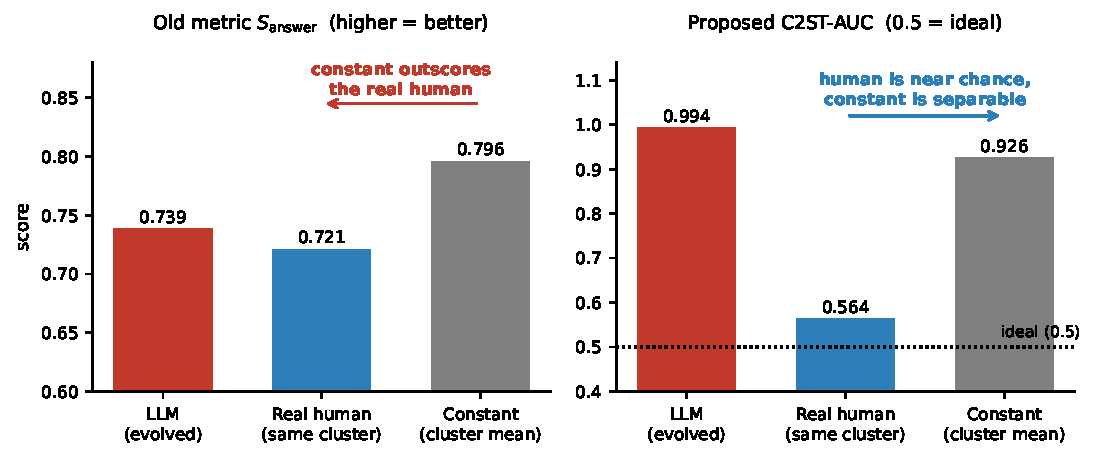
\includegraphics[width=\linewidth]{figures/inversion.pdf}
\caption{Corrected orientation, 20 cells. Left: under the old metric the
constant outscores a real human. Right: under C2ST-AUC (lower is better) the
human sits near chance ($0.5$) while model and constant are both highly
separable. Only the right panel places the human above the constant.}
\label{fig:inversion}
\end{figure}


\section{A distributional suite, and what it shows}
\label{sec:suite}

Before pricing anything we need a measurement maximised by distributional
fidelity rather than by central tendency, read against an explicit human
ceiling and constant floor. Three such measures --- a classifier two-sample
test, per-item distributional fidelity, and a variance ratio --- invert the
ranking correctly, placing humans above constants. Under them current
personas are near-perfectly separable from humans (C2ST-AUC $0.994$ against
a human ceiling of $0.564$) and reach only $0.43$ of human response
\emph{spread}. That spread shortfall is what \S\ref{sec:why} shows to govern
a persona's price, so it is the property the instrument quantifies rather
than merely flags. Appendix~\ref{app:suite} gives the definitions, anchors
and per-cell results.

\section{The same penalty, in a fitted decoder}
\label{sec:encoding}

The proposition concerns a faithful sampler against a constant. A fitted
predictor shows the same pressure. Fitting on half of each cluster and scoring
on the other half, two oracles differ only in what they emit: a \textbf{mean}
decoder (ridge on the ordinal code) predicting the conditional mean, and a
\textbf{residual-resampled} one, the same fit plus a resampled residual, which
restores marginal spread. The mean decoder scores $S=0.802$, the
residual-resampled one $S=0.730$ --- worse by $7.2$ points for being closer to
the response distribution on that margin. This is an illustration, not a test of Prop.~\ref{prop:main}: the decoder
conditions on a richer code than the belief prompts carry, so its $7.2$ points
are not a prediction of the $\mathrm{GMD}-\mathrm{MAD}$ gap. It beats the
constant ($0.792$) by $0.9$ points --- what one fitted reader achieved, not a
bound (App.~\ref{app:ceiling}).

% --- the strengthening campaign's new results -------------------------
% Everything above is the design rationale: the proposition establishes
% why a proper score is required, the audit establishes the scale of the
% miscalibration the price has to survive, and the fitted-decoder section
% establishes the baseline the price is quoted against.
% ===================================================================
% The answer-equivalent: definition, protocol, price, mechanism, boundary.
% Included from main.tex after the audit sections, which supply the
% design rationale for every choice made here.
% ===================================================================

\section{The answer-equivalent}
\label{sec:equiv}

\paragraph{Definition.} Let $S$ be a strictly proper ordinal score --- we use the
ranked probability score, normalised by the $K{-}1$ thresholds, so $S$ is
comparable across the $5$- and $7$-point inventories we study. Let a respondent
$i$ have observed answers $x_i$ and held-out answers $y_i$ on disjoint item sets.
Write $D_m$ for a conditional model fitted on training respondents that sees $m$
of respondent $i$'s observed answers, and $\widehat{F}$ for the simulator under
test. The answer-equivalent is
\[
m^{*}(\widehat{F})=\min\{m: \mathbb{E}\,S(D_m, y)\le \mathbb{E}\,S(\widehat{F}, y)\}.
\]
We report both this integer crossing, which is what a practitioner acts on, and
its linear interpolation between the bracketing budgets, which is the honest
effect size: the crossing is coarse and rounds a simulator up by as much as a
whole answer.

\paragraph{What the simulator is allowed.} $\widehat{F}$ is the persona readout
after population calibration; the raw readout scores worse than the population
prior, so pricing it raw would price the prompt format rather than the model. We
fit $\widehat{F}_{ij}=\Pi_{\mathrm{CDF}}[F_{0j}+\alpha(Q_{ij}-\bar{Q}_j)]$, with
$Q$ the model's own CDF from its digit logprobs, $F_0$ a population CDF fitted on
training respondents, $\bar{Q}$ its mean CDF on a calibration pool,
$\Pi_{\mathrm{CDF}}$ the exact $L_2$ projection onto monotone CDFs, and $\alpha$
chosen on calibration respondents. This is deliberately the most favourable
treatment: it hands the simulator a correctly located population distribution for
free and asks only whether its \emph{person-specific} deviations are worth
anything.

\paragraph{What the baseline is allowed.} $D_m$ is a ridge over the one-hot
observed answers onto the threshold indicators, projected onto monotone CDFs.
Its penalty is retuned at \emph{every} budget $m$, on the same calibration
respondents that select $\alpha$. This is not a detail: holding the penalty fixed
overfits the small budgets, and in development that alone manufactured an
apparent $15\%$ relative gain for the simulator at $m{=}100$ which vanished once
the baseline was tuned at each budget. A comparison across label budgets that
does not retune baseline capacity is measuring the baseline's misspecification.

\paragraph{Protocol.} Conditioning and target items are disjoint by
construction; respondents are split into a training block, a calibration half on
which every hyperparameter is selected, and an evaluation half on which every
reported number is computed frozen; uncertainty is a paired bootstrap over
evaluation respondents. Appendix~\ref{app:protocol} gives the full specification,
including the reverse-orientation correction, the common-support rule and the
multiplicity control.

\section{What a persona is worth}
\label{sec:price}

We price $89$ cells: every model in our artifact set, on IPIP-NEO-120, SD3,
IPIP-FFM-50 and HEXACO, on two disjoint respondent panels, plus the IPIP-NEO-300
unseen-item holdout of \S\ref{sec:transfer}.

\paragraph{The instrument is stable.} Across the $32$ (model, instrument) pairs
scored on both panels, $m^{*}$ on the \texttt{val} panel and on the \texttt{test2}
panel correlate at Spearman $\rho{=}0.78$ ($p{=}1.7\times10^{-7}$). The price is a
property of the model and instrument, not of a panel draw. Without this, nothing
below would be worth reporting.

\paragraph{The price.} Table~\ref{tab:ladder} gives the IPIP-NEO-120 ladder.
Median $m^{*}$ per inventory is $0.00$ on HEXACO, $0.06$ on IPIP-FFM-50, $0.32$
on IPIP-NEO-120, $0.40$ on SD3 and $0.61$ on the IPIP-NEO-300 holdout
(App.~\ref{app:equivfull}). The strongest persona we
measure on the short form is worth $3.07$ of $60$ answers; the weakest is worth
exactly zero, in the strong sense that calibration selects $\alpha{=}0$ and
discards its person-specific deviations entirely. Across all $89$ cells the median
is $0.19$ answers.

\begin{table}[t]\centering\footnotesize
\begin{tabular}{lrrr}
\toprule
Model & raw $S$ & $\alpha^{*}$ & $m^{*}$ (of 60)\\
\midrule
Qwen3.6-35B-A3B & 0.172 & 0.85 & \textbf{3.07}\\
Qwen2.5-32B & 0.213 & 0.30 & \textbf{2.15}\\
Qwen2.5-72B & 0.202 & 0.45 & \textbf{1.66}\\
Qwen3.8-27B & 0.183 & 1.10 & \textbf{1.31}\\
QwQ-32B-Preview & 0.202 & 0.70 & \textbf{1.29}\\
granite-4.2-30b & 0.243 & 0.45 & \textbf{0.45}\\
gemma-4-12B-it & 0.267 & 0.35 & \textbf{0.37}\\
Mistral-Small-24B-2501 & 0.324 & 1.00 & \textbf{0.33}\\
\midrule \multicolumn{4}{c}{\itshape 5 further models, App.~\ref{app:equivfull}}\\ \midrule
granite-4.1-8b & 0.356 & 0.20 & \textbf{0.02}\\
Apertus-8B-2509 & 0.286 & 0.00 & \textbf{0.00}\\
\bottomrule
\end{tabular}
\caption{Answer-equivalent on IPIP-NEO-120, averaged over both panels. $S$ is the
normalised ordinal RPS of the raw readout. $\alpha^{*}$ is the selected
calibration coefficient. Raw accuracy does not order the ladder;
$\alpha^{*}$ does.}
\label{tab:ladder}
\end{table}

\paragraph{Reading the number.} $3.07$ of $60$ is a real, replicable, non-zero
price, and it is small. Both halves matter. A practitioner with a $60$-item
instrument and a budget for three more questions should ask them. A practitioner
choosing between open models should read the ladder, because the spread across
models --- $0$ to $3.07$ --- is larger than any effect reported for prompt
optimisation on these systems.

\subsection{Transfer to an unseen item family}
\label{sec:transfer}

The splits above put every target facet's siblings in the conditioning half. The
IPIP-NEO-300 holdout removes that crutch: $300$ respondents answered the full
inventory, $120$ of whose items are exactly the short form used everywhere else,
and the other $180$ --- spanning all $30$ facets --- are items the same person
answered that no arm has been fitted on, with only $150$ training respondents
behind them. This is the thinnest supervision we measure and the most favourable
regime for a simulator, and it is where the price is highest: $\mathbf{5.38}$ of
$120$ answers, against $3.24$ of $60$ on the short form, with the model ordering
preserved. A persona is worth most exactly where human labels are scarcest.

Presentation matters as much as quantity. Given its persona as $m$ literal (item,
answer) pairs rather than a $30$-line profile, the same model prices at $0.00$,
$0.19$, $0.49$, $1.10$ for $m{=}5,20,60,120$ --- monotone, as it must be --- while
the profile built from those same $120$ answers is worth almost five times the
transcript of all of them ($\alpha^{*}$ $0.9$ against $0.3$). The direction is not
universal: Apertus-0.5B agrees ($0.13$ against $0.06$) but gemma-4-E2B reverses it
($0.22$ against $0.54$). Three models cannot settle which presentation wins; what
the price shows is that the choice is worth several observations and belongs in
the report (App.~\ref{app:transfer}).

\section{Why some personas are worth more}
\label{sec:why}

The ladder is not ordered by accuracy. The raw score of the best-priced model
($0.172$) and of \texttt{gpt-oss-20b} ($0.188$) are close, but their prices differ
by more than a factor of ten. Across all $89$ cells, raw score correlates with
$m^{*}$ at $\rho{=}-0.48$, and the \emph{calibrated} score --- the thing one would
naively report --- does not correlate with it at all.

What does order the ladder is $\alpha^{*}$, the share of a model's person-specific
deviation that survives calibration: $\rho{=}+0.72$ ($p{<}10^{-14}$), and
$\rho{=}+0.66$ after partialling out raw score. A model whose forecast barely
moves between people offers calibration nothing to keep; \texttt{Apertus-8B} has
$\alpha^{*}{=}0$ and a price of exactly zero, despite a middling raw score.

$\alpha^{*}$ is fitted against the same score $m^{*}$ is derived from, so on its
own it is a tight proxy rather than an independent cause. We therefore measured
the belief tensor directly, with no fitting and no labels. Controlling for raw
score, the \emph{entropy} of the model's person-conditional belief predicts the
price at $\rho{=}-0.52$ ($p{=}2.4\times10^{-7}$, $n{=}88$) while its marginal
correlation is null ($\rho{=}-0.03$): sharper conditional beliefs are worth more
real answers, independently of accuracy. Each step of the mechanism is then
measured rather than assumed --- sharper beliefs, larger person-specific
deviations, more of them surviving calibration, a higher price.

Between-person \emph{spread} of the belief does not predict the price
($\rho{=}+0.13$, $p{=}0.22$), nor do the cluster-level variance ratios of
\S\ref{sec:mechanism}. A population-level dispersion audit does not tell you what
a persona is worth to an individual; it is the sharpness of the conditional
belief, not the spread of the mixture, that carries the value.

\section{The boundary: personas are redundant given real answers}
\label{sec:boundary}

The price is quoted against a model given $m$ answers. The complementary question
is whether a persona adds anything to a model that already has \emph{all} of the
respondent's observed answers. It does not.

We screen $160$ cells. For each, three combination families are fitted on the
calibration half and frozen on the evaluation half: a convex weight between the
conditional model and the calibrated persona; a linear combiner taking the
persona's CDF as additional features beside the conditional model's; and a
gradient-boosted combiner over the same features. The control in each case is the
identical combiner, of identical capacity, fitted on identical rows, without the
persona features --- so the comparison isolates the persona and nothing else.

% eight columns do not fit one ACL column: as \begin{table} this overflowed the
% column by 98pt (about 1.4in of text in the margin). table* spans both.
\begin{table*}[t]\centering\footnotesize
\begin{tabular}{lrrrrrrr}
\toprule
Corpus & cells & LLM & prior & decoder & $\bar w^{*}$ & sig.\ cells & best $\Delta$\\
\midrule
HEXACO & 40 & 0.222 & 0.159 & 0.119 & 0.040 & 4/80 & +0.0001\\
IPIP-FFM-50 & 24 & 0.239 & 0.166 & 0.121 & 0.000 & 0/48 & +0.0000\\
IPIP-NEO-120 & 54 & 0.247 & 0.156 & 0.110 & 0.001 & 2/108 & +0.0000\\
SD3 & 42 & 0.215 & 0.167 & 0.130 & 0.000 & 2/84 & +0.0001\\
\bottomrule
\end{tabular}
\caption{Incremental value of a persona given the respondent's own observed
answers. $\bar w^{*}$ is the mean selected convex weight on the persona.
Significant cells are \emph{uncorrected} counts, shown to make the multiplicity
visible: across all $426$ one-sided tests, one survives Benjamini--Hochberg at
$q<0.05$, and it reverses sign on its own disjoint panel.}
\label{tab:incremental}
\end{table*}

The selected convex weight on the persona is $0$ in $127$ of $160$ cells, $0.05$
in the remaining $33$, and never higher. The linear combiner finds a nominally
significant positive increment in $0$ of $160$ cells. Across the full grid ---
$426$ one-sided tests --- $35$ are nominally significant at $5\%$, which is what
chance produces, and exactly \emph{one} survives Benjamini--Hochberg at $q<0.05$:
Qwen3.8-27B on HEXACO, \texttt{val} panel, gradient-boosted combiner,
$+0.00092$ $[+0.00046,+0.00140]$, $q{=}0.026$.

That cell does not survive scrutiny: on the disjoint \texttt{test2} panel the gain
reverses sign ($-0.00034$), and at four times the panel size it falls to
$+0.00006$ --- a small-sample artefact, as is every other nominally significant
HEXACO cell, all of which sit on the same $64$-respondent panel. We report it
rather than filter it out; a boundary claim that discards its one exception is
not a boundary claim.

This is a null reported as a null, not a failed superiority test: the combiner
gets every advantage its control gets, and it is the selected weight --- zero in
$127$ of $160$ cells --- rather than a $p$-value that concedes.

This is the sharp statement the price makes precise. A persona carries a small,
real, model-scaling amount of personal information --- and a handful of the
person's actual answers renders it redundant.


\paragraph{Beyond one questionnaire.} The structural defect is not a property of
IPIP-NEO-120. On the Short Dark Triad ($17{,}740$ respondents, $27$ items) the
same inequality holds on $27/27$ items, with a penalty of $8.67$ points against
IPIP's $7.75$, and the constant again outscores a real respondent ($0.744$ vs
$0.664$) in $200$ of $200$ bootstraps. \S\ref{sec:price} prices two further
inventories, IPIP-FFM-50 and HEXACO, on the same footing.

\section{Where the variance is lost}
\label{sec:mechanism}

The dispersion shortfall that \S\ref{sec:suite} measures has a locatable cause,
and it matters here because \S\ref{sec:why} shows a persona's price is governed
by exactly this quantity. Reading each model's own belief from its digit
logprobs, before any sampling, separates three stages: what the model believes,
what decoding emits, and what parsing recovers. The shortfall is already present
in the belief --- a low-dispersion model's forecast barely moves between
respondents, so there is nothing for decoding to discard and nothing for
temperature to reveal. Raising $T$ adds dispersion without adding alignment. All
mass lands on valid answer tokens throughout, so accounts blaming mode collapse
on difficulty \emph{emitting} numbers are unsupported. Appendix~\ref{app:variance}
gives the full ladder, the per-model tables and the reachability analysis.

Notably, the cluster-level statistics this analysis produces do \emph{not}
predict the individual-level price (\S\ref{sec:why}). A population dispersion
audit and an individual answer-equivalent are different measurements, and the
paper needs both.
\section{Related work}
\label{sec:related}

Personality conditioning of LLMs is validated by administering psychometric
inventories to the conditioned
model~\citep{serapio2023personality,jiang2024evaluating}, with well-documented
prompt sensitivity~\citep{han2026context,gupta2024personas}; simulation grounded
in interviews and self-reports achieves high individual
fidelity~\citep{park2026selfreports} at a per-person cost that motivates the
cluster-level shortcut, and evolutionary prompt
search~\citep{guo2024connecting,prasad2023grips,zhou2022large} supplies the
optimiser. That persona variables carry \emph{some} signal is already
established, and already quantified against supervised regression:
\citet{hu2024persona} find they explain under $10\%$ of annotation variance,
with persona prompting recovering about $81\%$ of what a regression on ground
truth achieves. Our question is the complementary one --- not whether the signal
exists, but what it is worth in answers. None of this literature reports that. Classifier two-sample
tests are standard for comparing
distributions~\citep{lopezpaz2017revisiting}, but the absolute-error objective
these systems optimise is minimised by a conditional central tendency, which is
why we anchor the price to a proper score instead.

Closest to us are methods that \emph{fix} simulator distributions rather than
price them: distributional fine-tuning on survey data~\citep{suh2025subpop},
two-stage shift alignment~\citep{huang2026dsa}, mean-preserving dispersion
adjustment over value profiles~\citep{abels2026valuepersonas} --- the family our
$\alpha$ belongs to --- and three-axis fidelity from small
pilots~\citep{choi2026beyondmean}. That calibration and distributional
fine-tuning are established is exactly why we claim neither; we contribute the
unit their gains should be quoted in. That work and behaviour-trained foundation
models~\citep{huang2026behaviorbench,binz2025centaur} target richer behaviour
than questionnaire response. Standardised group-level evaluation across many
datasets~\citep{hu2026simbench} is complementary to the price: it establishes
\emph{whether} a simulator matches a population, not how many of a person's
answers it substitutes for. The answer-equivalent applies to all of these
unchanged wherever a held-out response distribution exists.

\section{Conclusion}

We priced respondent simulators in the currency a practitioner spends: questions
asked of a real person. The answer-equivalent is stable across disjoint panels,
orders models consistently, and is governed by how much person-specific deviation
survives calibration rather than by accuracy. The strongest open persona we
tested is worth $5.38$ of $120$ answers on an unseen item family and the weakest
exactly zero, and across $160$ cells a persona adds nothing to a model that
already holds the respondent's own answers. The instrument is what we ask the
field to adopt: it makes ``our simulator is better'' a claim with units.

\section*{Limitations}

Our audit covers one corpus (IPIP-NEO-120), one clustering pipeline, one
optimisation family, and five models; the belief-level measurement of
\S\ref{sec:mechanism} covers eleven open-weight models spanning 7B--235B,
six families and three generations, and the cross-instrument replication
carries the structural findings and the identity
result but not the full suite, which needs sampled
simulator outputs where SD3 has only the two belief readouts of
App.~\ref{app:disjoint}; belief-level measurement anywhere needs logprob access
the API models in the audit do not provide, and three current large
mixture-of-experts models --- GLM-5.3-Flash, Qwen3.8-Flash-Next and
DeepSeek-V4-Flash --- could not be read at all on this protocol, returning NaN
or zero mass on the answer tokens or shipping no chat template, so the
candidate pools here reach $35$B and not beyond; individual readouts are
reproducible bit-for-bit across clusters and software stacks but \emph{not}
across accelerator architectures, where $7.7\%$ of modal answers flip, so the
per-item beliefs we release should be read as machine-specific even though the
aggregates they feed move by at most $0.016$ (App.~\ref{app:repro}); the within-family trend rests on three
points and the cross-family comparison on eleven, so both are directional rather
than fitted laws; all models are read with thinking disabled and the assistant
turn prefilled, and the four least confident of them (belief entropy above $1$
nat) should not have their above-human total dispersion read as calibrated
uncertainty, though low confidence cannot inflate
$\mathrm{VR}_\text{between}$, which is computed from persona means; two
elicitation details proved to matter more than we expected --- reading these
models through a chat-completions server returned almost no mass on the answer
tokens where the forward pass recovers $0.99$--$1.00$, and harmony-format models
require the assistant turn to open a channel before the prefill, without which
mass on the scale falls to $0.39$ --- so a null result in this literature may
report a readout rather than a model; precision varies across the models we
report --- nine run at bf16, gpt-oss-20b ships MXFP4 and is dequantised to bf16 at
load, and Qwen3-235B is an FP8 checkpoint served at FP8 --- and a further FP8
checkpoint resisted measurement through both available routes, so we make no
claim that individuation is invariant to quantisation; the proposition is general
to the
absolute-error metric in \eqref{eq:metric}, but the empirical magnitudes are
specific to this setting. The model answers we re-score were produced by prior
runs we did not control, at temperatures we did not set, and one released run was
committed with entirely missing answers and is excluded. Our human ceiling is a
single same-cluster respondent, which underestimates what a well-specified
individual-level twin could achieve; we make no claim about individual-level
methods. C2ST-AUC depends on classifier capacity and on $n{=}40$ per side, so its
absolute value should be read as a lower bound on separability, and
\S\ref{sec:c2st-audit} shows most of what it reads is response style; we fold the
AUC as $\max(\mathrm{AUC},1-\mathrm{AUC})$, which places the null above $0.5$
($0.517$ signed against $0.569$ folded) and makes our small-$n$ floor a property
of this classifier rather than of C2ST; and DF treats
items independently and so ignores within-respondent answer dependence. The
corpus is self-reported, skewed toward respondents aged 18--25 and toward the
USA, UK and Canada, so neither the clusters nor the ceilings should be read as
representative of any broader population.

Limits specific to the price. (i) $m^{*}$ is a threshold crossing on a curve
estimated with noise; we report the interpolated value and a paired bootstrap on
the loss gap, but a single cell's crossing is fragile --- the top cell's gap
excludes zero on one panel and not on the other, which is why we lead with the
ladder and the cross-panel rank correlation rather than with any one number.
(ii) $\alpha^{*}$ is fitted against the same score $m^{*}$ is derived from, on a
disjoint respondent half but the same objective, so it is a tight proxy for
retained person-specific deviation rather than an independent cause of it.
(iii) The price is quoted against the specific conditional model we use; a
stronger conditional model would lower every $m^{*}$, so our numbers are upper
bounds on what a persona is worth. (iv) We price questionnaire response, not
behaviour. The four corpora are four disjoint populations with no shared
respondents, so we cannot demonstrate that one person's identity transfers
across behavioural domains, and we make no such claim. (v) The data contain one
response per person--item cell and no repeated administration, so we cannot
estimate the irreducible response noise that bounds any simulator, and $m^{*}$
therefore cannot be expressed as a share of attainable performance.
(vi) Our null results are reported as nulls under a pre-specified comparison with
Benjamini--Hochberg control across the $426$-test grid, but we did not
pre-register an equivalence margin, so ``adds nothing'' should be read as
``adds nothing detectable at this sample size and effect scale''.

Finally, we show that current personas are worth little on this instrument; we do
not show that no method can be worth more, and the instrument is designed to
register it when one is.

\section*{Ethics statement}

We use a public, de-identified corpus of self-reported personality questionnaire
responses and add no new human-subjects data collection. Our results are
cautionary: they indicate that current cluster-level personality simulations are
readily distinguishable from real respondents and under-represent human response
variance, and so should not be used as substitutes for human participants in
research, product, or policy decisions. Reporting an evaluation number without
its constant floor risks overstating the fidelity of synthetic respondents, which
is the specific harm this paper aims to reduce. Simulating demographic or
personality groups also risks reinforcing stereotypes when cluster descriptions
are treated as characterisations of real people rather than as statistical
summaries.


\appendix

\section{Reproducibility}

Every analysis in this paper is deterministic given its inputs and requires no
LLM calls except the belief-level measurement of \S\ref{sec:mechanism}. The
released corpus and committed run artefacts reconstruct the scoring, selection
and orientation analyses. Some inputs are too large for the repository and are not in it: the refreshed
belief tensors behind App.~\ref{app:current}, the per-respondent score arrays
behind App.~\ref{app:reach}, the $n{=}512$ forecast tensors behind
App.~\ref{app:rules}, and the cross-cluster and cross-architecture replication
readouts behind App.~\ref{app:repro}. These accompany the submission as one
archive ($568$ files, $92$\,MB compressed) carrying a per-file SHA-256 manifest
and the CPU commands that regenerate each number above from it; no GPU and no
model weights are required, because the archive holds the saved model outputs
rather than the runs that produced them. We verified that path end to end: from
the archive alone, the intervals of App.~\ref{app:current}, the frequencies of
App.~\ref{app:reach}, the eight paired differences of App.~\ref{app:rules} and
the deviations of App.~\ref{app:repro} all reproduce as printed. We do not claim
the list is exhaustive; where an analysis consumes a tensor, the tensor is in
the repository only if this appendix says so, and otherwise in the archive. We ran the full analysis pipeline
independently on two clusters with different operating systems, Python versions
and library versions (scikit-learn 1.2 vs 1.7, pandas 2.1 vs 3.0). Every reported
figure we compared --- the $\lambda^\star$ values, the orientation deltas, the
variance components, and the null-calibration ARIs of App.~\ref{app:clusters} ---
agreed to the digits we print, except the $k{=}4$ reproduction ARI, which is
$0.946$ on one environment and $0.951$ on the other. Code and per-cell results are released. The belief simplices
$(40\text{ personas}\times120\text{ items}\times5)$ per cluster are included for
the eleven models of \S\ref{sec:mechanism}, with the persona ordering fixed by
the released corpus. Runs that failed
the validity guard ship too, marked invalid, so the record shows what was
measured and rejected. One transform maps model answers onto the corpus's
recoded scale and is imported by every analysis that compares the two.

\section{A disjoint conditioning/target replication}
\label{app:disjoint}

Every belief result in the body conditions on scores computed from the same
items it is then scored on, so a sceptic can say the models reconstruct
arithmetic rather than predict a person. We remove that by construction. Items
are split within each scale, the persona is built only from the input half, and
the readout covers only the target half: two input and two target items per IPIP
facet ($60$/$60$), four input and five target per SD3 trait ($12$/$15$). No
cluster label is used --- the released IPIP clustering is derived from all $120$
items and would reimport target information --- and the prior and the decoder are fitted on training
respondents whose target answers are never seen. The five score bins are fixed
equal-width bands of the $0$--$100$ range, not fitted. This design differs from the
body's in more than the split: the persona is one generated line per facet
rather than the body's per-cluster prose, respondents are sampled globally
rather than within clusters, and only half the items are scored. It is a
replication under a stricter design, not a controlled ablation of overlap.

On $256$ held-out respondents the second fact of \S\ref{sec:mechanism} is
unqualified and the first is weakened. Every model still loses to the empirical
prior, by $0.098$--$0.204$ across all four model--instrument cells. The identity
effect survives in three of those four: on SD3 by $+0.010$ $[+0.006,+0.016]$ for
Qwen2.5-7B and $+0.017$ $[+0.013,+0.020]$ for Granite-4.1, and on IPIP by
$+0.004$ $[+0.002,+0.005]$ for Qwen2.5-7B --- but Granite-4.1 on IPIP gives
$+0.002$ $[-0.001,+0.005]$, which does not exclude zero.

One thing follows and one does not. Positive identity gains occur with
conditioning and target items disjoint, in three of four cells, so item overlap
is not necessary for them. What this design cannot do is apportion the body's
IPIP gain between overlap and identity, because it changes the persona text, the
respondent sample and the scored items as well as the split: Qwen2.5-7B's
$0.006$ there and $0.004$ here are not two measurements of one quantity, and an
interval excluding zero in one design beside one that does not in another is no
evidence of a decrease. What survives every cell is that the simulator loses to
a prior that ignores the persona.

\section{Does the replacement change a decision?}
\label{app:selection}

An audit that only condemns a metric leaves the practical question open: if
you adopt the replacement, do you ship something different, and is it better?
We fix one candidate set and select twice.

Candidates are the eleven belief models of \S\ref{sec:mechanism}, re-run under
the disjoint-item prompts of App.~\ref{app:disjoint}; the body's readouts
cannot serve, since they condition on scores computed from the answers being
scored. Qwen3-235B is excluded: its FP8 checkpoint read correctly on one
allocation and returned near-zero mass on the answer tokens on others, so it
fails the same $\ge 0.5$ mass criterion we apply throughout, and reading it
through a different execution path would give one candidate an elicitation
route the other ten did not have. Both rules see the same probability
forecasts, never greedy answers: rule~A ranks by expected answer similarity,
the audited $S_0$; rule~B by $S_{1/2}$. Selection uses $128$ respondents;
evaluation uses $128$ more, disjoint from those, from the $20{,}000$ training
respondents on which both baselines are fitted, and from App.~\ref{app:disjoint}'s
panel. Only the selected models are run on the evaluation panel.

The rules disagree. Rule~A selects Qwen2.5-72B ($S_0=0.753$); rule~B selects
Qwen3.5-9B ($L_{1/2}=0.187$) --- models an order of magnitude apart in size. On
the untouched panel rule~B's pick is better by $0.010$ $[0.004,0.016]$ under
$L_{1/2}$ (lower is better), paired over respondents. The task is ordinal prediction, so that is
the outcome we report; categorical log-loss agrees and is secondary, at $1.37$
nats $[1.26,1.48]$. The log-loss gap is the larger number but the weaker
argument, since it mostly registers the 72B's overconfidence rather than its
ordinal accuracy --- its errors are confident, not distant. Its one advantage
is independence: neither selection rule uses log-loss, whereas $S_{1/2}$ is
rule~B's own criterion, evaluated on disjoint respondents.

Two caveats belong with this. It is one candidate set, one split and one
instrument, so it shows the evaluation changed a decision for the better ---
not that it reliably does. And the improvement is relative: both picks lose to
the training-fitted empirical prior ($0.155$, $1.41$ nats), so the replacement
recommends a smaller model and simultaneously reports that no candidate beats
ignoring the persona. Adding the degenerate candidates makes the point sharper
still. With the constant vector in the pool, rule~A selects \emph{it} over
every model ($S_0=0.766$ against the 72B's $0.753$), which is
Prop.~\ref{prop:main} arriving as a deployment recommendation; rule~B
selects the prior. The constant's log-loss is infinite, and we report it as
such rather than clipping it.

\section{Which scoring rule selects best?}
\label{app:rules}

App.~\ref{app:selection} compares two rules on one instrument, and says plainly
that this cannot show the replacement \emph{reliably} chooses better. Here we
widen it: nine scoring rules, twelve open-weight models spanning $0.5$B to
$35$B across six families, and four instruments, two of which the body never
uses.

The rules span three classes. Strictly proper: $S_{1/2}$ (ranked probability
score), Brier, log-loss, spherical. Weakly proper: RMSE of the forecast mean,
and mode accuracy. Improper: the audited $S_0$, MAE of the forecast mean, and
Wasserstein distance to the observed point mass, which coincides with $S_0$ by
construction here and so is not independent evidence. Instruments are IPIP-NEO-120,
SD3 and IPIP-FFM-50 on five points, and HEXACO-PI-R on \emph{seven} --- the
last is the only place the pipeline is exercised at $K\neq5$. The first three
are keyed from published item keys; the HEXACO distribution we use ships none,
so its reverse-keyed items are inferred from each item's correlation with the
rest of its scale, and HEXACO results carry that caveat. Each rule selects on
$512$ respondents and is graded on $512$ disjoint others, with baselines fitted
on a further $8{,}000$; all $96$ readouts put at least $0.92$ of their mass on
the answer tokens.

We score a selector by the \emph{regret} its pick incurs, normalised within the
candidate set so $0$ is the best of these twelve models and $1$ the worst, and
averaged over the strictly proper evaluators \emph{excluding the selector's own
rule}, so no rule is graded on the criterion it optimised. Because eight rules
are compared against one reference, we report Holm-adjusted $p$ and Bonferroni
simultaneous intervals, and call a difference resolved only when both agree.
The four differences below with intervals excluding zero all carry Holm
$p\le0.01$; the three strictly proper alternatives carry $p=1.00$.

\begin{center}\small
\setlength{\tabcolsep}{3.5pt}
\begin{tabular}{@{}llr@{\,}l@{}}
\toprule
rule & class & \multicolumn{2}{c}{regret vs.\ $S_{1/2}$ (Bonferroni CI)}\\
\midrule
RMSE of mean & weak & $+0.000$ & $[+0.000,+0.000]$\\
Brier & strict & $+0.003$ & $[-0.008,+0.025]$\\
log-loss & strict & $+0.004$ & $[-0.007,+0.022]$\\
spherical & strict & $+0.007$ & $[-0.002,+0.029]$\\
MAE of mean & improper & $+0.025$ & $[+0.007,+0.055]$\\
mode accuracy & weak & $+0.238$ & $[+0.084,+0.262]$\\
$S_0$ audited & improper & $+0.298$ & $[+0.250,+0.368]$\\
Wasserstein & improper & $+0.298$ & $[+0.250,+0.368]$\\
\bottomrule
\end{tabular}
\end{center}

Each row grades the two selectors on the same evaluators --- the strictly
proper rules minus both contestants' own criteria --- so a rule is never
compared on a set containing its opponent's criterion but not its own.
Differences are bootstrap means over respondents, $B{=}4000$; intervals are
Bonferroni simultaneous bounds holding jointly over all eight comparisons. Every improper rule selects worse than
$S_{1/2}$, and the audited $S_0$ is the worst of them. The gap is not marginal:
mean regret is $0.259$ for $S_0$ against $0.003$ for $S_{1/2}$. On SD3, $S_0$
selects a model whose regret is $0.98$ --- all but the worst of the twelve ---
while every strictly proper rule selects the best. An evaluator using the
audited metric on this pool would ship very nearly the worst simulator
available.

The number depends on the pool. With eight closely matched instruction-tuned models the same comparison
gives $+0.028$ $[+0.011,+0.059]$: still resolved, ten times smaller. Regret is
normalised within the candidate set, so it measures position within that pool
and cannot be read across pools. What it does show is where in \emph{this}
pool the audited metric lands: near the bottom on SD3, where its selection
carries regret $0.98$, while the proper rules select the best.

Three things this does not say. The strictly proper rules remain mutually
indistinguishable, so the evidence is for the class boundary, not a ranking
inside it. RMSE of the forecast mean --- only weakly proper --- is not
distinguishable from $S_{1/2}$ at all: it selects the same model on every
instrument, and its paired difference is exactly zero. Eliciting the mean is
sufficient on this candidate set, and we have no basis for preferring a strict
rule over it. And regret is normalised within the candidate set, so $0$ means
the best of these twelve, never good: every candidate still loses to the
persona-free prior of App.~\ref{app:disjoint}.

Mode accuracy is the other collapse, at $+0.238$. Discarding the distribution
and keeping the argmax is as damaging as the metric this paper audits. If a
practitioner takes one operational rule from this work, it is that a simulator
must be scored on the distribution it induces, not on the answer it would most
likely give.

Sample size decided the weaker version of this. At $128$ respondents per panel
with eight candidates the $S_0$ comparison was $+0.070$ $[-0.017,+0.273]$ ---
unresolved. Quadrupling the panels resolved it; widening the pool made it
large.

\section{When does impropriety actually bite?}
\label{app:whenbites}

App.~\ref{app:rules} shows $S_0$ selecting all but the worst simulator from a
heterogeneous pool. It would be convenient to conclude that optimising $S_0$ is
therefore harmful wherever it appears. We tested that directly and it is false.

The system this paper audits was built by evolving cluster-level system prompts
to maximise $S_0$. We take those evolved genotypes and the base genotypes the
search started from, assemble both with the original code, and read the same
belief distribution under each --- scoring with the objective that was
optimised and with two proper rules. The prediction we registered before
running was that $S_0$ would improve while the proper scores would not.

\begin{center}\small
\setlength{\tabcolsep}{4pt}
\begin{tabular}{@{}lr@{\,}r@{\,}r@{}}
\toprule
model & $\Delta S_0$ & $\Delta L_{1/2}$ & $\Delta$log-loss\\
\midrule
Qwen3.8-27B      & $+0.060$ & $-0.039$ & $-0.235$\\
granite-4.2-8B   & $+0.046$ & $-0.046$ & $-0.630$\\
gpt-oss-20b      & $+0.052$ & $-0.043$ & $-0.251$\\
gemma-4-12B-it   & $+0.070$ & $-0.068$ & $-0.619$\\
\bottomrule
\end{tabular}
\end{center}

Evolved minus base, $256$ held-out respondents over four clusters, paired
bootstrap. Every interval excludes zero and \emph{every} direction is an
improvement: $L_{1/2}$ and log-loss are losses, so the negative signs are
gains. The prediction is falsified on all four models. Across respondents the
change in $S_0$ and the change in $S_{1/2}$ correlate at $r=0.96$--$0.99$, and
$85$--$97\%$ of respondents improve on both at once.

The two results are not in tension. $S_0$ is maximised by a constant vector
(Prop.~\ref{prop:main}) --- a \emph{point mass}, not a flat distribution --- so
its optimum is under-dispersed. Writing $\bar\sigma$ for a model's mean
predictive standard deviation, the Spearman correlation between $S_{1/2}$ as a
reward and $\bar\sigma$ is positive on all four instruments ($+0.71$ to
$+0.86$): the proper score consistently prefers the more dispersed candidate.
$S_0$ does not, and its correlation varies --- $+0.03$ on IPIP, $-0.09$ on
IPIP-FFM, $-0.40$ on HEXACO and $-0.97$ on SD3 --- with the failure tracking
the penalty. On SD3, where the correlation is $-0.97$, $S_0$ ships a model with
$\bar\sigma=0.48$ against the proper rule's $1.10$ and incurs regret $0.98$; on
IPIP and IPIP-FFM, where it is near zero, both rules select the same model and
the regret is zero. These are correlations over twelve candidates per
instrument and we read them as descriptive, not as an identified mechanism.

What we can say about optimisation is narrower. Evolutionary prompt search
improved both $S_0$ and the proper scores on all four models tested, so
optimising an improper objective did not degrade the artefact here. We have
since measured the dispersion of the candidates a prompt search can visit
(App.~\ref{app:reach}): over twelve persona conditions the rules disagree on
two models of four, and on one of those the disagreement is stable under
resampling, with $S_0$ taking the less dispersed candidate. The degenerate
direction is therefore reachable by prompt search in this candidate set, at a
small observed cost. Model selection over a heterogeneous pool is the other
case we measured: an over-confident weak model is already most of the way to a
point mass, so $S_0$ rewards it and ships it.

The pattern across the two settings is narrower than ``never optimise $S_0$''.
In the candidate sets we measured, $S_0$ disagreed with a proper rule far more
visibly in the model-selection pool, where it shipped a near-worst simulator,
than in the prompt pool, where the selected candidates scored within
$0.001$ CRPS of each other. We do not convert that into a claim that one setting
is more dangerous than the other: the two are not measured on a common scale
(App.~\ref{app:reach}). We report
this because it bounds our own claim: the audit establishes that $S_0$ is
improper and that it selects badly, not that every system built with it is
worse for having used it.

\section{Is a belief readout a measurement?}
\label{app:repro}

Every number in App.~\ref{app:rules} treats a readout as a stable property of a
model. That is an assumption, and this paper's own Limitations record the
readout \emph{path} moving mass on the answer tokens from $0.39$ to $0.99$, so
we tested it rather than appealing to determinism. Two models and two
instruments were re-read with the same script, seed and respondent panels on
independent systems.

\paragraph{Same architecture and dtype, different everything else.} Between two
clusters running different software --- torch $2.11.0$ with transformers
$5.17.0$ against torch $2.13.0$ with transformers $5.16.1$, both on H200 and
both on the \texttt{bf16} path --- the readouts are \emph{bit-identical}:
maximum deviation $0$ over the full belief simplex and $0$ of $76{,}800$
item--respondent pairs changing their modal answer. This is a statement about
two small models on one numeric path, and \S\ref{app:mixedpath} below shows it
does not extend to a change of dtype.

\paragraph{Different architecture.} Against A100 (sm\_80) instead of H200
(sm\_90), on the same \texttt{bf16} path, they are not. Mean absolute deviation
per probability is $0.008$--$0.029$, and $5{,}946$ of $76{,}800$ modal answers
flip --- $7.7\%$. The divergence is not a mismatched comparison: the four cells
score identical respondents, and the flips sit precisely on near-ties. Where a
modal answer flips, the median gap between the model's top two levels is
$0.051$ against $0.507$ where it does not; for one cell that median gap is
$0.000$, exact ties resolved differently by different kernels.

\paragraph{What survives.} The scores largely do. Averaged over the four
cells, the change is $1.6\times10^{-3}$ for $S_0$, $3.4\times10^{-3}$ for mode
accuracy and $4.7\times10^{-3}$ for $S_{1/2}$; the largest single-cell change
is $1.6\times10^{-2}$, for $S_{1/2}$ on gemma-4-E2B/SD3. We do not convert
these into a ratio against the regret differences of App.~\ref{app:rules}: raw
score changes and candidate-range-normalised regrets are different units and
the comparison would be meaningless. What we can say is bounded and direct ---
a change of architecture moves a model's score by at most $0.016$ here, while
it moves $7.7\%$ of that model's individual answers.

We had expected the distribution-based scores to be the \emph{stable} ones,
which would have given \S\ref{sec:suite} a second argument independent of
propriety. They are the least stable of the three, and we report that rather
than the argument we went looking for. The practical reading is narrower: a
per-item LLM ``belief'' is not reproducible across accelerators and should not
be published as though it were, while an average over hundreds of items and
respondents is stable enough to carry an effect an order of magnitude larger
than the noise.

One arm was initially missing from \emph{this} comparison: V100 (sm\_70) tests
the \texttt{fp16} path, and the build we first used ships no Volta kernels, so
the comparison above spans two Hopper-class and one Ampere-class device only.
The \texttt{fp16} path is the path on which part of \S\ref{sec:mechanism}'s table
was measured. We fill that arm below.

\subsection{The table is not on a single numeric path}
\label{app:mixedpath}

Auditing the run records for \S\ref{sec:mechanism} showed that its rows were not
all produced on one device class. \texttt{h4\_variance\_ladder\_hf.py} selects
\texttt{bf16} at sm\_80 and above and \texttt{fp16} below it, and four rows ---
Mistral-Small-24B, Qwen2.5-7B, Qwen2.5-32B and QwQ-32B --- were read on V100
(sm\_70) in \texttt{fp16}, while the remainder were read on H200 (sm\_90) in
\texttt{bf16}. The appendix above tests \texttt{bf16} against \texttt{bf16}; it
never tested the path those four rows used.

We therefore re-read all four on sm\_90 in \texttt{bf16}, holding the model, the
script, the panel ($40$ personas per cluster) and the respondents fixed, so that
only the device class and dtype differ. The belief readout is deterministic
given a model and a panel --- the seed enters only the sampled answers --- so
these are not repeated draws:

\begin{center}\scriptsize
\setlength{\tabcolsep}{4pt}
\begin{tabular}{lccc}
\toprule
Model & sm\_70 \texttt{fp16} & sm\_90 \texttt{bf16} & $\Delta$\\
\midrule
Qwen2.5-7B & 0.430 & 0.427 & $-0.003$\\
Qwen2.5-32B & 0.343 & 0.340 & $-0.003$\\
QwQ-32B & 0.753 & 0.824 & $\mathbf{+0.070}$\\
Mistral-Small-24B & 0.579 & 0.771 & $\mathbf{+0.192}$\\
\bottomrule
\end{tabular}
\end{center}

Two of the four reproduce to $0.003$ in $\mathrm{VR}_\text{total}$. Two do not:
QwQ moves $9\%$ and Mistral $33\%$, in both cases because the model emits
flatter answer distributions on the newer path --- Mistral's mean belief entropy
rises from $0.729$ to $0.984$ --- which inflates the within-persona term. Panel
size is not the explanation: on sm\_90 Mistral moves $0.002$ between $40$ and
$160$ personas.

\paragraph{The \texttt{fp16} arm, and one row that does not reproduce.}
The missing V100 arm above was attributed to a build without Volta kernels. That
is a property of the build, not of the hardware: a different interpreter
available on the same cluster (torch 2.6.0+cu124) runs on sm\_70, so we re-read
all four \texttt{fp16}-origin rows on V100 in \texttt{fp16}, holding model,
script, panel and respondents fixed. Three reproduce their published values to
$10^{-4}$ in both columns --- Qwen2.5-7B $0.1931$ against $0.193$, Qwen2.5-32B
$0.2204$ against $0.220$, QwQ-32B $0.1538$ against $0.154$ in
$\mathrm{VR}_\text{between}$ --- and each published value falls inside a
$2000$-replicate persona bootstrap interval. This is the first measurement of
\emph{within}-path drift rather than an assumption of it, and it puts that drift
at or below $10^{-4}$, one to three orders of magnitude under the cross-path
deltas above.

Mistral-Small-24B does not reproduce. Its re-read gives
$\mathrm{VR}_\text{between}=0.1619$ $[0.1481,0.1678]$ against a published
$0.177$, which lies outside the interval, with
$\mathrm{VR}_\text{total}$ $0.5733$ against $0.579$ and mean belief entropy
$0.758$ against $0.729$. The discrepancy is not run-to-run noise and not device
sharding: two independent re-reads on two and on three V100s return
\emph{bit-identical} belief tensors. Some unrecorded aspect of the original
Mistral run therefore differs from the configuration its record describes, and
we cannot say which, because the artifacts of that era do not carry the device,
dtype or library versions that produced them --- a gap our released readouts now
close. We report the figure as not reproduced rather than silently replacing it;
the cross-path contrast for this model should be read from the reproducible
endpoint ($0.5733$ on \texttt{fp16} against $0.771$ on \texttt{bf16}), which
leaves its direction and rough magnitude unchanged.

\paragraph{The individuation column is not affected.} The quantity
\S\ref{sec:mechanism} actually rests on is $\mathrm{VR}_\text{between}$, and it
survives the change of path where the total does not. Re-reading ten of the
eleven rows on sm\_90 \texttt{bf16} at a common $160$-persona panel (QwQ at
$40$, the largest panel on which it returns a readout) reproduces every
published $\mathrm{VR}_\text{between}$ to within $0.0064$, and the four
\texttt{fp16}-origin rows are no worse than the six \texttt{bf16}-origin ones:

\begin{center}\scriptsize
\setlength{\tabcolsep}{2.5pt}
\begin{tabular}{lccc}
\toprule
Model & pub. & re-read & $\Delta$\\
\midrule
Qwen2.5-7B$^\dagger$ & 0.193 & 0.187 & $-0.006$\\
Qwen2.5-32B$^\dagger$ & 0.220 & 0.221 & $+0.001$\\
Qwen2.5-72B & 0.295 & 0.292 & $-0.003$\\
Mistral-24B$^\dagger$ & 0.177 & 0.176 & $-0.001$\\
QwQ-32B$^\dagger$ & 0.154 & 0.148 & $-0.006$\\
gpt-oss-20b & 0.126 & 0.123 & $-0.003$\\
Granite-4.1-8B & 0.207 & 0.203 & $-0.004$\\
Apertus-8B & 0.130 & 0.125 & $-0.005$\\
GLM-4.7-Flash & 0.265 & 0.263 & $-0.002$\\
Qwen3.5-9B & 0.167 & 0.163 & $-0.004$\\
\bottomrule
\end{tabular}
\end{center}

\noindent$^\dagger$ published row measured on sm\_70 \texttt{fp16}.

Mistral is the clearest case: its $\mathrm{VR}_\text{total}$ moves $0.192$
between paths while its $\mathrm{VR}_\text{between}$ moves $0.001$. That is what
the mechanism predicts. A change of numeric path alters how sharp each
persona's answer distribution is, which is a within-persona quantity; it barely
moves where those personas' \emph{means} sit, which is what
$\mathrm{VR}_\text{between}$ measures.

The practical consequence is narrower than the mixed path first suggests. The
individuation claims of \S\ref{sec:mechanism} and the ordering of models by
$\mathrm{VR}_\text{between}$ stand: every published value reproduces within
$0.0064$ on one path. What does not transfer is the total-dispersion column and
the within/between share derived from it, for the two models whose distributions
sharpen. We leave the published table as measured and flag the affected
statistic rather than restating numbers, and note that
App.~\ref{app:current} is uniformly sm\_90 \texttt{bf16} throughout.

One further caution for anyone reusing the script: at $160$ personas the QwQ
read returned \texttt{NaN} for every cell while exiting normally, and was caught
only by the validity guard that rejects an all-missing run. The same read at
$40$ personas succeeded. We have not traced the cause; a partially rather than
wholly degenerate version of that fault would not trip the guard.

\section{Split sensitivity of the baselines}
\label{app:split}

Re-drawing which 100 respondents are sampled at a
fixed 60/40 ratio moves the parameter-free cluster-mean baseline by
$0.54$--$0.77$ points within a cluster over 20 draws, and the four-cluster
average by $0.23$ (pooling clusters gives $1.33$, mixing cluster differences into
split variation). Prior work's gain is $+0.72$ points on one fixed split. This is
context for how far a split can move a score, not a test of that gain: variation
in baseline \emph{levels} does not bound a \emph{paired} improvement.

\section{What is a persona worth, in respondents?}
\label{sec:equivalents}

``It loses to a constant'' invites the reply that the constant is a strawman. So
we restate the finding in a unit that is harder to dismiss: how many real
respondents you would have to sample before a plug-in estimate of the cluster's
response distribution matches what the persona gives you.

Drawing $m$ real respondents, forming the per-item empirical distribution, and
sampling a synthetic population from it yields distributional fidelity $0.723$ at
$m{=}1$, $0.797$ at $m{=}2$, $0.915$ at $m{=}21$ and $0.923$ at $m{=}34$. The
curve is evaluated at the same sizes as the audited scores --- forty synthetic
against forty held-out humans --- because DF depends on sample size, so a curve
built at any other size cannot calibrate them. Reading the audited systems off
it:

\begin{center}\footnotesize
\setlength{\tabcolsep}{4pt}
\begin{tabular}{lcc}
\toprule
System & DF & Resp.-equiv.\\
\midrule
Evolutionary LLM persona & 0.783 & \textbf{2}\\
Constant cluster mean & 0.795 & 2\\
Human ceiling & 0.939 & off-curve\\
\bottomrule
\end{tabular}
\end{center}

An evolutionary-optimised persona is worth about \textbf{two} real respondents:
two is the smallest evaluated $m$ whose mean DF exceeds the persona's $0.783$,
and the constant sits at the same place. This is a threshold on the mean curve,
not an equivalence test. The human ceiling of $0.939$ is not crossed anywhere on
the evaluated grid, up to $m{=}500$ ($0.938$), so we do not convert it into
respondent units --- a statement about the grid we searched, not a proof that no
$m$ reaches it. This is the same result
as \S\ref{sec:audit} in different units, and it is the version we would put to a
practitioner weighing synthetic respondents against a small pilot survey.

\section{The C2ST feature ladder}
\label{app:c2staudit}

A metric that separates simulators from humans at AUC $0.994$ invites an obvious
objection: perhaps the classifier is detecting formatting rather than anything
about personality. We test our own metric with a feature ladder, each rung scored
identically against the same anchors. Orientation is handled per feature family:
style features describe how a respondent uses the scale, so both sides sit on the
literal scale the item was asked on, while content features compare
trait-oriented quantities. The full-item rung reproduces the suite's $0.994$.

\begin{center}\footnotesize
\setlength{\tabcolsep}{4pt}
\begin{tabular}{lccc}
\toprule
Features & LLM & Human & Const.\\
\midrule
Full 120 items & 0.994 & 0.564 & 0.926\\
5 style scalars only & 0.894 & 0.584 & 0.988\\
Items, ipsatised & 0.989 & 0.566 & 0.986\\
30 facet scores only & 0.991 & 0.565 & 0.908\\
Forward-keyed only & 0.990 & 0.568 & 0.810\\
Reverse-keyed only & 0.993 & 0.583 & 0.843\\
\bottomrule
\end{tabular}
\end{center}

Five content-free scalars --- per-respondent mean and standard deviation, extreme
-response rate, longest identical run, and forward-versus-reverse consistency ---
attain $80\%$ of the full above-chance AUC on their own. The objection has real
force, and we state it plainly: \textbf{response style alone reproduces most of
the separability}, which is a statement about what suffices, not a decomposition
of what the full classifier uses.

It is not only style. Ipsatising each respondent (removing their own mean and
standard deviation, i.e.\ the two largest style features) still leaves AUC
$0.989$, and facet scores alone give $0.991$. Style and content are redundant
routes to the same conclusion rather than one masking the other. The human
ceiling is also stable at $0.56$--$0.58$ across every rung, so the anchor does
not move with the feature set.


\section{Cluster validity in full}
\label{app:clusters}

Since stability-based model selection is common, the general point is worth
stating: at large $n$, bootstrap agreement must be read against a
covariance-matched null or it certifies nothing.

No \emph{separation} criterion supports $k{=}4$. Silhouette falls overall from
$0.134$ at $k{=}2$ to $0.053$ at $k{=}15$, with minor upward steps, taking
$0.082$ at $k{=}4$;
Davies--Bouldin is also minimised at $k{=}2$; the gap statistic increases
monotonically and selects no interior $k$. A silhouette below $0.1$ indicates
essentially no separated structure.

\emph{Stability} looks at first like a defence: bootstrap ARI over 40 resamples
is $0.977$, $0.952$, $0.932$, $0.903$ at $k{=}2,3,4,5$ and falls away after
($0.797$, $0.581$), so $k{=}4$ looks close to the largest reproducible $k$.

That reading does not survive a null calibration. Rebuilding the pipeline on
structureless surrogates --- a Gaussian matched to the real $30\times30$ facet
covariance, and a copula matched to the covariance and every per-facet marginal
--- reproduces the stability number exactly: ARI $0.911$ and $0.921$ at
silhouette $0.075$ and $0.078$, against the real data's $0.910$ at $0.082$. A
separated 4-component control confirms the test has power (silhouette $0.672$,
ARI $1.000$).

At $n{=}410{,}168$ any smooth unimodal cloud with this covariance is partitioned
reproducibly, so ARI $\approx0.91$ measures estimator variance, not multimodality,
and neither criterion supports $k{=}4$. The clusters are not demographic
artefacts either (Cram\'er's $V$ of $0.055$--$0.057$ against sex, age band and
country); they are a reproducible discretisation of a continuum, which bounds the
cluster-conditional signal any persona can exploit. Since stability-based model
selection is common, the general point is worth stating: at large $n$, bootstrap
agreement must be read against a covariance-matched null or it certifies
nothing.


\section{What the persona channel carries}
\label{app:ceiling}

A persona reaches the model only through \texttt{get\_modifier\_bisect}, which
writes each score as one of five words on width-20 bins; each cluster's genotype
names five traits and five of the thirty facets, and every other sentence of the
system prompt is shared. Ten words therefore carry the respondent's identity, and
two respondents sharing those ten bins would receive byte-identical prompts and
so must receive identical beliefs.

We estimate what that channel permits. Within each cluster we fit
$\mathbb{E}[X_j \mid \text{code}]$ on respondents \emph{excluding} the forty
personas, then evaluate on those forty, so the quantity is directly comparable to
$\mathrm{VR}_\text{between}$ and is never fitted on its own evaluation set.

\begin{center}\footnotesize
\setlength{\tabcolsep}{3pt}
\begin{tabular}{@{}p{0.72\columnwidth}r@{}}
\toprule
Conditioning available to the model & Dec.\ SD\\
\midrule
Ten scores, five words \emph{(audited system)} & 0.482\\
\quad same, with boosted trees & 0.483\\
Ten scores, written as numbers & 0.512\\
All 35 scores, five words each & 0.707\\
All 35 scores, written as numbers & 0.726\\
\midrule
\textit{best of the eleven} & \textit{0.295}\\
\bottomrule
\end{tabular}
\end{center}

Three things follow. The quantisation is not the binding constraint: writing
numbers instead of words buys $0.03$. The channel is not degenerate: all forty
personas in all four clusters receive distinct codes, so no model is forced to
answer two personas identically. And a boosted-tree decoder, which can use interactions, lands in the same place
($0.483$ against $0.482$); that is consistent with the additive fit being close
to the conditional mean, though two similar SD ratios do not prove it.

The oracle is fitted on this population and so knows its code-to-response
mapping, which a zero-shot model does not; we therefore do not claim that a model
\emph{ought} to reach $0.482$. The comparison rules out one explanation only ---
that the conditioning carries too little information to individuate --- and that is
the explanation the flatness of $\mathrm{VR}_\text{between}$ across eleven
models most invites.

\paragraph{Uncertainty in \S\ref{sec:mechanism}.} Identity gain and the prior
comparison use $2000$ percentile-bootstrap draws over respondents, $40$ per
cluster with equal cluster weight. The permutation control is not sampled but
computed exactly, as the expectation of every donor row against every
respondent; the prior and decoder are fitted once on the excluded respondents and
held fixed, so intervals cover respondent sampling, not fitting.

\paragraph{Uncertainty on $A$.} Persona rows are resampled jointly across the
model, the decoder and the actual respondents, so paired comparisons stay
paired; the decoder fit is held fixed, so the intervals describe
persona-sampling uncertainty rather than fit uncertainty. Over $2000$ draws the
human reference is $0.498$ $[0.461,0.517]$ and the eleven models span $0.033$
$[0.028,0.036]$ for Apertus-8B to $0.183$ $[0.168,0.193]$ for Qwen2.5-72B. The
intervals are informative enough to separate models that
$\mathrm{VR}_\text{between}$ ranks together: Qwen2.5-32B and Granite-4.1 differ
by $0.013$ in spread but their amplitudes do not overlap, $[0.105,0.122]$
against $[0.071,0.089]$. Comparisons are made on the paired draws, not by asking whether marginal
intervals overlap --- two overlapping marginals can still have a difference
interval excluding zero, as GLM-4.7 and Qwen3-235B do ($+0.017$
$[+0.009,+0.025]$) --- and Qwen2.5-32B exceeds Granite-4.1 by $+0.034$
$[+0.028,+0.040]$ despite a $0.013$ gap in spread.

\paragraph{Where the shortfall falls.} Each cluster names five facets, so twenty
items have their own facet stated and one hundred are covered only at trait
level. The named items carry $1.51\times$ more predictable-from-code signal (an SD ratio)
(reference $0.671$ against $0.444$), and $10$ of $11$ models individuate them more
in absolute terms, Qwen3-235B being the exception ($0.224$ named against $0.264$
elsewhere). Measured against those references the ratio is \emph{lower}
where the prompt is most specific --- $0.353$ on the named items against $0.433$
on the rest, in the same direction for $10$ of $11$ models --- but we report this
descriptively and draw no causal conclusion from it, for two reasons. A facet
score is computed from its own four items, so $\mathbb{E}[X_j\mid\text{facet}]$
is close to an arithmetic identity that a model without the scoring key cannot
invert, while traits have the same structure diluted over twenty-four items; the
named-item reference is inflated by more than the trait-level one, which alone
could produce the gap. And the eleven models share personas, references and
prompt structure, several within one family, so they are not independent
replicates and we do not attach a $p$-value to the count.

\paragraph{Widening the channel does not fix it.} The obvious remedy is to send
more: we re-ran three models with every other word of the prompt held fixed and
the ten modifier phrases replaced by the numbers themselves. The effect is
inconsistent in magnitude --- $\mathrm{VR}_\text{between}$ rises for Granite-4.1
($0.207\!\to\!0.246$) and gpt-oss ($0.126\!\to\!0.146$) but falls for Apertus
($0.130\!\to\!0.096$) --- and, using the same joint draws so the comparison is
paired, every model moves resolvably: $A$ shifts by $+0.053$
$[+0.045,+0.059]$ for Granite-4.1 and $+0.008$ $[+0.005,+0.012]$ for gpt-oss but
$-0.013$ $[-0.016,-0.009]$ for Apertus. The effect is therefore not noise; it is
real and model-dependent in sign. It is also inconsistent in direction, the aligned
amplitude moving $0.081\!\to\!0.134$ for Granite-4.1 and
$0.039\!\to\!0.047$ for gpt-oss but $0.033\!\to\!0.020$ for Apertus. Granite
gains on both counts --- its correlation with the oracle rises from $0.285$ to
$0.453$ --- so for that model the richer encoding is a real improvement, while
Apertus loses spread and direction together. On three models a richer encoding
is therefore a plausible but unreliable remedy, and we report it as a pilot
rather than a recommendation.

\paragraph{The alignment does not depend on the oracle.} Because $r$ is measured
against a fitted target, an oracle missing structure the models track would
understate it. It does not. Boosted trees on the same code change $r$ by at most
$0.012$ and a ridge on the continuous scores by at most $0.034$; an oracle given
all thirty-five scores lowers $r$ substantially, by up to $0.168$, which is the
expected direction since models only ever see the ten-score code. The ordering of
models is unchanged throughout. Two independent computations agree where theory
demands it: the ceiling as a standard-deviation ratio is $0.482$ and the oracle's
correlation with actual respondents is $0.491$, which coincide for a conditional
mean. The check that assumes no oracle at all --- correlating each model's persona
means directly against the forty respondents' own answers --- gives
$0.076$--$0.248$ against the oracle's $0.491$, so models recover between a sixth
and a half of the attainable person-level alignment.

\section{Current-generation models, with intervals}
\label{app:current}

The eleven-model table in \S\ref{sec:mechanism} predates three of the four
families below; gpt-oss-20b is re-measured rather than new. We repeated the belief-level measurement on one current model
from each, under the identical protocol ($40$ personas per cluster, four
clusters, exact readout from the retained probability vectors), and added the
interval the original table lacks. Some readouts are missing for
Gemma-4 --- $30$ persona--item readouts of $19{,}200$, one in $640$, all in
cluster~1 where they are $30$ of $4{,}800$ (coverage $0.99375$); those cells
are held out of the moments rather than summed to zero, which would enter as an
impossible answer of $0$ and inflate the between-persona term. Every other model
here has complete coverage. Resampling is over personas --- the
exchangeable unit for a between-persona variance --- with $2000$ draws; because
the protocol assigns the same personas to every model, each replicate applies
one set of persona indices to all four, so the differences below are paired.

\begin{center}\scriptsize
\setlength{\tabcolsep}{2.5pt}
\begin{tabular}{lcccc}
\toprule
Model & Params & VR$_\text{with}$ & VR$_\text{betw}$ [95\% CI] & VR$_\text{tot}$\\
\midrule
Granite-4.2-8B & 8B & 0.729 & \textbf{0.155} [0.143, 0.160] & 0.757\\
Gemma-4-12B-it & 12B & 0.336 & \textbf{0.334} [0.303, 0.345] & 0.506\\
gpt-oss-20b (MoE) & 21B & 1.120 & \textbf{0.127} [0.118, 0.130] & 1.130\\
Qwen3.8-27B & 27B & 0.869 & \textbf{0.219} [0.197, 0.229] & 0.911\\
\midrule
\textit{human} & --- & --- & 1.000 & 1.000\\
\bottomrule
\end{tabular}
\end{center}

\paragraph{The measurement replicates.} gpt-oss-20b appears in both tables from
independent runs. The new run returns $\mathrm{VR}_\text{between}=0.127$ against
$0.126$, $\mathrm{VR}_\text{within}$ $1.120$ against $1.121$, and
$\mathrm{VR}_\text{total}$ $1.130$ against $1.131$. We report this because it is
our only same-model repeat under this variance protocol (App.~\ref{app:repro}
tests readout stability separately), and it bears on \S\ref{sec:mechanism}
rather than on the new models.

\paragraph{The $0.30$ bound is not a law.} Gemma-4-12B measures
$\mathrm{VR}_\text{between}=0.334$ $[0.303,0.345]$, above the $\approx0.30$
figure that held across all eleven earlier models --- but the interval's lower
end sits essentially \emph{at} that figure, so we read this as evidence that the
ceiling is a property of the models we happened to measure rather than as a
decisive refutation of it. The qualitative claim is unchanged: $0.334$ is still
about a third of the human value. We have scoped
\S\ref{sec:mechanism} accordingly rather than restating the bound as universal.

\paragraph{The two failure modes are separable.} Gemma-4 and gpt-oss-20b fail in
opposite directions, and the intervals separate them. gpt-oss-20b carries
\emph{above}-human total dispersion ($\mathrm{VR}_\text{total}=1.130$) of which
almost none individuates: the between-persona share of belief variance is
$0.016$ $[0.014,0.018]$. Gemma-4 is its mirror --- a between-persona share of
$0.504$ $[0.466,0.524]$ but collapsed in magnitude
($\mathrm{VR}_\text{total}=0.506$). It is not alone in that: Qwen2.5-32B and
Qwen2.5-72B in the eleven-model set have between-persona shares of $0.485$ and
$0.429$. The paired difference, gpt-oss minus Gemma-4, is
$-0.488$ $[-0.507,-0.451]$. Near-human total spread is therefore not evidence of
individuation, and individuation is not evidence of human-like spread; a single
variance ratio cannot distinguish the two, which is the argument of
\S\ref{sec:mechanism} restated on models chosen after it was written.

\paragraph{What does not separate.} Of the six paired comparisons of the
between-persona share, five exclude zero and one does not: Granite-4.2 against
Qwen3.8 is $-0.008$ $[-0.017,+0.003]$. Their point estimates, $0.068$ and
$0.076$, must not be read as an ordering. We note it because the same two models
\emph{do} separate on $\mathrm{VR}_\text{between}$ itself ($-0.064$
$[-0.073,-0.049]$): which quantity is reported decides whether these two models
are distinguishable, and the point estimates alone would not have revealed that.

\section{Is the degenerate direction reachable by prompt search?}
\label{app:reach}

App.~\ref{app:whenbites} reports that prompt search improved $S_0$ and the
proper scores together, and notes that this alone cannot establish whether the
degenerate optimum is out of reach --- we had not measured the dispersion of the
candidates a search can actually visit. This appendix measures it.

\paragraph{Design.} We cross six persona directives with the base and evolved
genotypes, giving twelve candidates scored on the same $192$ respondents.
Three directives are intended to push towards concentration (\textit{decisive}: avoid
middle-of-the-scale answers; \textit{extreme}: answer at the ends;
\textit{consistent}: similar items receive the same number), one is intended to push towards
spread (\textit{varied}), one asks for the spread of a single real respondent
(\textit{calibrated}), and one is the unmodified prompt. Each candidate is
scored under $S_0$ and under CRPS, and we record its mean predictive SD. The
verdict is fixed in code before the run: \textsc{reachable} iff the candidate
$S_0$ selects is strictly less dispersed than the one the proper rule selects.

\paragraph{Stability.} A strict inequality between two close candidates is not a
result, so we resample respondents ($2000$ draws, paired --- all conditions are
scored on the same respondents) and \emph{re-run the selection inside each
replicate}, so the reported stability includes the selection uncertainty rather
than freezing the point-estimate picks.

\begin{center}\scriptsize
\setlength{\tabcolsep}{3pt}
\begin{tabular}{lccc}
\toprule
Model & $S_0$ selects & rules differ & \textsc{reach.}\\
\midrule
Granite-4.2-8B & evolved/varied & $0\%$ & $0.0\%$\\
Gemma-4-12B-it & evolved/varied & $0\%$ & $0.0\%$\\
Qwen3.8-27B & evolved/varied & $77\%$ & $77.4\%$\\
gpt-oss-20b & evolved/calibrated & $99\%$ & $\mathbf{99.2\%}$\\
\bottomrule
\end{tabular}
\end{center}

\paragraph{Two point-estimate disagreements; one of them stable.} On Granite-4.2
and Gemma-4 both rules select the same candidate in every one of the $2000$
replicates: nothing to separate. On Qwen3.8 the point estimate fires
\textsc{reachable}, but the proper rule's own choice is unstable --- it takes
\textit{calibrated} in $77\%$ of replicates and \textit{varied} in the rest ---
so we report it as inconclusive rather than as a second instance. On
gpt-oss-20b the disagreement is stable: $S_0$ selects \textit{evolved/calibrated}
in $100\%$ of replicates, CRPS selects \textit{evolved/varied} in $99\%$, the two
rules differ in $99.2\%$, and $S_0$'s candidate is less dispersed by $0.0453$
$[0.0439,0.0465]$. That is the phenomenon Prop.~\ref{prop:main} predicts, produced
by an ordinary prompt search rather than by a constructed counterexample.

\paragraph{What these frequencies are, and are not.} The $90\%$ stability line
that separates ``stable'' from ``inconclusive'' above is a descriptive cut we
chose, not an inferential guarantee. It is not load-bearing: gpt-oss alone
qualifies at $80$, $90$, $95$ and $99\%$, and neither disagreement qualifies at
$99.5\%$. A bootstrap selection frequency is the stability
of a choice under resampling, not the probability that a claim is true. The
resampling is stratified to match the design --- $48$ respondents drawn within
each of four clusters, as H21 draws them --- but re-selecting inside each
replicate measures selection instability on one evaluation panel, which is not
an independent deployment test. We therefore read App.~\ref{app:reach} as an
exploratory finite-candidate result.

\paragraph{The cost of following it is small.} Magnitude matters for the
practical claim. On gpt-oss-20b the contested pair is
\textit{evolved/varied} ($S_0=0.7173$, CRPS $=0.1667$, $\bar\sigma=0.899$)
against \textit{evolved/calibrated} ($S_0=0.7234$, CRPS $=0.1677$,
$\bar\sigma=0.854$). Following $S_0$ costs $0.0010$ of CRPS --- about $0.6\%$ of
the better candidate's score --- and buys a $5\%$ reduction in dispersion. So the
degenerate direction is reachable here, but the observed cost of taking it is
small. We deliberately do not compare that figure to the $0.98$ regret reported
for model selection in App.~\ref{app:whenbites}: that regret is normalised
within a candidate set and averaged over evaluators, and this is a raw CRPS
difference, so the two are not on one scale. What the two experiments jointly
show is that the disagreement occurs in both settings, not that one is
quantifiably more dangerous than the other.

\paragraph{The directives that ask for confidence do not deliver it.} Across all
four models neither \textit{decisive} nor \textit{extreme} is selected by either
rule, and both \emph{lower} $S_0$ relative to the unmodified prompt. The reason
is not that they concentrate in the wrong place: measured against the matching
base prompt they \emph{raise} mean predictive SD in $13$ of $16$ model--genotype
comparisons. Their names describe an intention, and the measured effect usually
runs the other way, so we report them as instruments that failed rather than as
evidence about where $S_0$'s optimum lies. \textit{Calibrated}, which $S_0$ selects on gpt-oss, asks for the spread of a
single real respondent rather than for confidence. It is not the only condition
that lowered dispersion --- \textit{evolved/varied} sits below
\textit{evolved/base} on all four models, and both rules select it on Granite-4.2
and Gemma-4. A search that reliably
produced low-dispersion candidates might well find more disagreement than we do;
our directive set is a weak probe of that space.

\section{Finite-sample behaviour of the anchors}
\label{app:samplesize}

Both anchors are estimated from $n{=}40$ per side, which for a classifier over
120 features is a small-sample regime. We sweep $n$ on human-only data, where the
true answers are known: two disjoint samples from the same cluster must be
indistinguishable, so the honest C2ST value is exactly $0.5$ and any excess is
estimator bias.

\begin{center}\scriptsize
\setlength{\tabcolsep}{3pt}
\begin{tabular}{lcccccc}
\toprule
$n$ & 20 & 40 & 80 & 160 & 320 & 640\\
\midrule
C2ST human & --- & 0.574 & 0.542 & 0.536 & 0.527 & 0.517\\
DF human & 0.915 & 0.939 & 0.957 & 0.969 & 0.978 & 0.985\\
C2ST const. & --- & 0.914 & 1.000 & 1.000 & 1.000 & 1.000\\
\bottomrule
\end{tabular}
\end{center}

Two corrections follow, in opposite directions, and both land on their
theoretical values. Fitting $y = y_\infty + c\,n^{-1/2}$ over the non-degenerate
range gives an extrapolated C2ST human ceiling of $\mathbf{0.500}$ and an
extrapolated DF human ceiling of $\mathbf{1.000}$ --- exactly what two samples
from the same distribution must score. So the C2ST ceiling of $0.574$ at $n{=}40$
is \emph{entirely} finite-sample classifier bias and should be read with its $n$
attached, while the DF ceiling of $0.939$ is \emph{entirely} plug-in Wasserstein
bias and is pessimistic. Correcting the latter widens the gap to the simulator's
$0.783$ rather than narrowing it.

Below $n\approx40$ \emph{this} classifier stops separating even the constant from
real humans (the dashed entries above are the degenerate $0.5$). That floor is a
property of the configuration we used, not of C2ST: relaxing the minimum leaf
size from $20$ to $5$ restores separation at $n{=}20$. We therefore recommend
reporting every anchor together with the $n$ and the classifier settings it was
measured at, and treating any small-$n$ floor as something to establish per
configuration rather than to inherit from us.


\section{Where the variance is lost, in full}
\label{app:variance}


Knowing the simulator is mis-dispersed does not say \emph{where} the dispersion
goes. We read the model's own belief before any sampling occurs, on open-weight
models served locally.%


\paragraph{Two stages.} For each persona and item we take the model's
next-token distribution over the answer tokens $\{1,\dots,5\}$ directly from the
logprobs, then sample each item from its own belief and score the resulting
population. One implementation detail matters: hybrid reasoning models emit a
\texttt{<think>} token first --- with probability $\approx 1$ --- so a naive
readout sees no mass on the scale at all; we disable thinking and prefill the
assistant turn.

\paragraph{Result.} What is collapsed is the \emph{individuating} part of the
belief, not the belief's total spread. In the 2024--25 models both are small;
in the 2026 reasoning-first models the total spread reaches or exceeds the
human marginal while individuation stays as low as ever.

The statistic matters. The quantity comparable to a human
\emph{across-respondent} SD is not the average within-persona conditional SD but
the SD of the persona-\emph{mixture} distribution, from the law of total
variance $\mathrm{Var}(X_j)=\mathbb{E}_i[\mathrm{Var}(X_j\mid i)]
+\mathrm{Var}_i(\mathbb{E}[X_j\mid i])$, computed exactly from the retained
probability vectors. The within-persona term alone would understate a faithful
simulator, which can hold sharp per-persona beliefs and still match human
variance through differing persona means.

\begin{center}\scriptsize
\setlength{\tabcolsep}{2.5pt}
\begin{tabular}{lcccc}
\toprule
Model & Params & VR$_\text{with}$ & VR$_\text{betw}$ & VR$_\text{tot}$\\
\midrule
Qwen2.5-7B-Instruct & 7B & 0.367 & \textbf{0.193} & 0.430\\
Qwen2.5-32B-Instruct & 32B & 0.242 & \textbf{0.220} & 0.343\\
Qwen2.5-72B-Instruct & 72B & 0.367 & \textbf{0.295} & 0.488\\
Mistral-Small-24B & 24B & 0.538 & \textbf{0.177} & 0.579\\
QwQ-32B (reasoning) & 32B & 0.729 & \textbf{0.154} & 0.753\\
Qwen3-235B-A22B-2507 & 235B & 0.695 & \textbf{0.258} & 0.758\\
Qwen3.5-9B & 9B & 1.058 & \textbf{0.167} & 1.078\\
GLM-4.7-Flash (MoE) & 29B & 1.209 & \textbf{0.265} & 1.242\\
gpt-oss-20b (MoE) & 21B & 1.121 & \textbf{0.126} & 1.131\\
Granite-4.1-8B & 8B & 0.386 & \textbf{0.207} & 0.457\\
Apertus-8B-Instruct & 8B & 0.927 & \textbf{0.130} & 0.939\\
\midrule
\textit{human} & --- & --- & --- & 1.000\\
\bottomrule
\end{tabular}
\end{center}

Essentially all probability mass lands on the five valid answer tokens
($0.97$--$1.00$), so no model has difficulty \emph{emitting} a number. Belief
entropy nonetheless spans $0.42$--$1.38$ nats (maximum $\ln 5 = 1.609$), and we
can offer no clean account of it: it tracks neither release date (Granite-4.1,
$0.49$) nor reasoning-tuning (QwQ $0.97$; the standard-instruct Apertus $1.24$).
The 235B model is the one the audited system used, so this measures that system,
not a proxy.

\paragraph{Total dispersion and individuation are decoupled.} The decomposition
says something the total does not, and the evidence for this is existential
rather than correlational. gpt-oss-20b and Qwen2.5-72B invert cleanly: the
former has $2.3\times$ the total dispersion of the latter ($1.131$ vs $0.488$)
and \emph{less than half} its individuation ($0.126$ vs $0.295$). The rank
correlation over the eleven models is $\rho=-0.30$ with a bootstrap 95\%
interval of $[-0.92,0.42]$.

QwQ-32B sharpens it: its dispersion is almost all per-item uncertainty ($0.729$
of $0.753$), and it individuates less ($0.154$) than far smaller models.

The Qwen2.5 family isolates this at fixed family and varying scale:
individuation rises monotonically, $0.193 \to 0.220 \to 0.295$ at 7B, 32B, 72B,
while the total does not, moving $0.430 \to 0.343 \to 0.488$.

One bound survives across the whole set --- a $34\times$ parameter range, six
families, three generations, dense and mixture-of-experts, and both standard and
reasoning-tuned models: no model here exceeds
$\mathrm{VR}_\text{between}\approx0.30$ --- a bound on this set, not a law:
Gemma-4-12B, measured later, reaches $0.334$ (App.~\ref{app:current}).
Individuation stays under half the human
value throughout, and neither the largest model nor the most dispersed one is
the best at it.

\paragraph{The persona helps, and still loses.} Two questions have run together:
does the simulator reproduce the cluster's distribution, and does it identify
\emph{this} respondent? Scoring each persona against that person's own answers
under normalised CRPS, and permuting belief rows among respondents within a
cluster --- which leaves every population statistic identical while destroying
identity --- separates them. All eleven score better on the correct assignment
than the permuted one by $0.004$--$0.017$, every paired interval excluding zero,
yet all remain worse than a cluster empirical prior fitted on \emph{other}
respondents --- which uses cluster membership but no persona --- by
$0.036$--$0.095$. With conditioning and target items disjoint, the gain is
resolved in three of four tested cells and unresolved for Granite-4.1 on IPIP,
while all four still lose to the prior (App.~\ref{app:disjoint}).

The two facts reconcile exactly, and without any fitted reference. Writing $I$
for the identity gain above, $\bar q$ for the model's within-cluster mean CDF and
$D_Q$ for the across-persona variance of its CDFs,
\begin{equation}
R(P_0)-R(Q)\;=\;I\;-\;D_Q\;-\;\big[R(\bar q)-R(P_0)\big],
\label{eq:decomp}
\end{equation}
an identity in measured quantities, exact on our data to machine precision. It
locates the loss. The bracket --- how much worse the model's \emph{mixture} is
than the prior --- is $0.038$--$0.090$, whereas the net identity contribution
$D_Q-I$ lies within $\pm0.005$ for every model, in absolute value below a tenth
of that model's mixture excess. Spread across personas can help or hurt
slightly; what decides the comparison is that the mixture itself is wrong.

\paragraph{The prompt is not what caps individuation.} A persona is individuated
only through a five-word quantisation of ten numbers, but that channel carries
more than the models extract: a supervised conditional-mean decoder fitted on
held-out respondents reaches $0.482$ on these same personas, where the best model
delivers $0.295$, and no two personas share a code (App.~\ref{app:ceiling}). The
decoder is a reference, not a bound --- a mis-calibrated simulator could exceed it
by dispersing wrongly --- so it shows the conditioning carries signal.

\paragraph{How much of it points the right way.} $\mathrm{VR}_\text{between}$
measures how far apart a simulator places its persona means, not whether that
spread identifies the right respondent. Correlating each model's persona means
against the oracle's over the forty personas --- both on the corpus's recoded
scale --- gives $r=0.16$--$0.52$. The aligned amplitude
$A=\frac{1}{J}\sum_j r_j\,\mathrm{sd}(M_j)/\mathrm{sd}(H_j)$, in units of human
item SD, is $0.033$--$0.183$, against $0.498$ $[0.461,0.517]$ for real
respondents: the best reaches about a third of that, the weakest under a tenth.
It separates models $\mathrm{VR}_\text{between}$ ranks together --- GLM-4.7 and
Qwen3-235B sit $0.007$ apart in spread, yet differ in $A$ by $+0.017$
$[+0.009,+0.025]$ --- and rises with scale across Qwen2.5 in three
non-overlapping steps ($0.067\to0.116\to0.183$).

A simulator can therefore look more dispersed simply by being less confident:
$\mathrm{VR}_\text{total}$ confounds uncertainty with individuation, and
$\mathrm{VR}_\text{between}$ is what a persona claim should be judged on.

Total dispersion is not uniformly low: it is $0.758$ for the largest
2024--25 model and exceeds the human marginal for three others ($1.078$,
$1.131$, $1.242$). Nor is it lost at decoding: sampling retains almost all of
it ($1.078\!\to\!1.061$, $1.243\!\to\!1.218$, $1.131\!\to\!1.115$). What stays
limited at every scale is \emph{individuation}.

For the low-dispersion models the spread is likewise not discarded at
decoding; it was never present, so recovering it there means \emph{adding}
dispersion, not revealing it: $p^{1/T}$ lifts Qwen2.5-7B from
$0.43$ to $1.02$ at $T{=}5$ while supplying none of the alignment $A$ measures.
And since all mass lands on valid answer tokens, accounts blaming mode collapse
on difficulty \emph{emitting} numbers are unsupported here.


\section{Is $k{=}4$ a partition at all?}
\label{app:kfour}


The audited systems condition on a $k{=}4$ $k$-means partition of the 30 facet
scores. We reproduce it (ARI $=0.946$) and test $k\in\{2,\dots,15\}$ under three
preprocessings: no criterion supports $k{=}4$, and the bootstrap stability that
appears to defend it is matched exactly by structureless surrogates
(App.~\ref{app:clusters}). The clusters are a convenient partition, not a
discovered structure --- which is why our results are stated for the partition
the systems use rather than for personality types.


\section{What is C2ST actually reading?}
\label{app:c2streading}

\label{sec:c2st-audit}

A metric that separates simulators from humans at AUC $0.994$ invites the
objection that the classifier detects formatting rather than personality. A
feature ladder (App.~\ref{app:c2staudit}) shows the objection has real force:
five content-free response-style scalars already recover most of the separability
above chance. It is not only style --- ipsatising each respondent, or using facet
scores alone, still separates nearly as well --- so style and content are
redundant routes to the same conclusion. We therefore recommend reporting C2ST with its style-only rung alongside it, so
readers can see how much of any separability is carried by response style. A
simulator that closed only the style gap would look far better on the headline
number while remaining just as distinguishable on content.

The anchors are estimated at $n{=}40$ per side. Appendix~\ref{app:samplesize}
sweeps $n$ and shows the C2ST human ceiling is entirely finite-sample classifier
bias (extrapolating to $0.500$) while the DF ceiling is entirely plug-in bias
(extrapolating to $1.000$, i.e.\ pessimistic). Below $n\approx40$ our classifier
configuration stops separating at all, so we report every anchor with the $n$ and
the settings it was measured at rather than proposing a universal floor.


\section{Cluster conditioning, per cell}
\label{app:permutation}


No persona study we know of reports the wrong-persona control, so no reported
persona effect is currently attributable to the persona. We score every simulator
against every cluster's humans --- 80 cells --- and report diagonal dominance
descriptively.

\begin{center}\footnotesize
\setlength{\tabcolsep}{5pt}
\begin{tabular}{lccc}
\toprule
Metric & Matched & Mismatched & $\Delta$\\
\midrule
$S$ & 0.728 & 0.663 & $+0.065$\\
DF & 0.782 & 0.705 & $+0.077$\\
C2ST & 0.996 & 0.985 & $-0.010$\\
VR & 0.431 & 0.436 & $-0.005$\\
\bottomrule
\end{tabular}
\end{center}

Matched comparisons improve $S$ and DF; they show no improvement in C2ST or VR.
We report these gaps descriptively and attach no $p$-value: a permutation that
shuffles the 80 cell labels freely destroys the matched structure of the five
$4\times4$ matrices, and the models share clusters and personas, so its null is
not the right one. Rescoring fixed outputs against different human populations
also does not isolate a causal effect of changing the prompt. This is the behavioural counterpart of
\S\ref{sec:suite} --- the persona moves which items get endorsed, and not who is
endorsing them --- and it makes the wrong-persona control as necessary a baseline
as the constant floor.


\section{Answer-equivalent protocol in full}
\label{app:protocol}

Conditioning and target items are disjoint by construction,
split within each scale, so the simulator is never scored on items its persona
was built from. Respondents are split three ways: a training block on which
$F_0$, the prior and every $D_m$ are fitted; a calibration half of the scored
panel on which $\alpha$, the ridge penalty and any combination weight are
selected; and an evaluation half on which every number we report is computed,
frozen. Uncertainty is a paired bootstrap over evaluation respondents. Where the
corpus stores reverse-recoded answers --- IPIP-NEO-120 does, on $43$ of $60$
targets; SD3 does not --- the model's simplex is reversed on those items before
scoring. Omitting that step is invisible in every variance statistic and wrong in
every score.

\section{The orientation audit in full}
\label{app:orientation}


Before comparing anything, the two sides must be on the same scale. They are not.

The released corpus stores human answers \emph{reverse-recoded} so that a higher
number always means more of the trait, while the simulator is shown the literal
item text --- ``Cheat to get ahead'' --- and asked how accurately it describes
it, i.e.\ it answers \emph{raw}. On the $55$ negatively-keyed items of the
IPIP-NEO-120 the two scales run in opposite directions, and every published
model-vs-human comparison is computed across that flip.

Two signatures make this unambiguous. Negatively-keyed items average $3.373$
against $3.425$ for positively-keyed ones --- level, whereas raw self-reports on
undesirable content sit far lower. And ``Cheat to get ahead'' carries a human
mean of $4.15$ out of $5$.

The effect is large and it runs \emph{against} the simulator. Correcting the
orientation raises the correlation between the model's and the humans' per-item
mean profiles from $+0.09$ --- indistinguishable from no relationship at all ---
to $+0.63$, and raises $S$ from $0.660$ to $0.739$.

Three conclusions survive, with their invariances:

\begin{itemize}\itemsep1pt
\item \textbf{Proposition~\ref{prop:main} is invariant.} $\mathrm{MAD}$ and
$\mathrm{GMD}$ are computed on the human distribution alone, and both are
reflection-invariant.
\item \textbf{The variance ratio is exactly invariant}, since
$\mathrm{sd}(6-x)=\mathrm{sd}(x)$. The under-dispersion finding of
\S\ref{sec:suite} is untouched.
\item \textbf{The constant still wins every cell.} Reorientation closes the gap
from $13.6$ to $5.8$ points, but the constant cluster mean beats the corrected
model in $20$ of $20$ cells.
\end{itemize}

Correcting the defect in fact \emph{sharpens} the paper's claim. The corrected
model scores $0.739$, \emph{above} the $0.721$ of a real member of the target
cluster --- while a classifier separates that same model from real members at AUC
$0.994$ (\S\ref{sec:suite}). A metric that ranks a near-perfectly detectable
simulator above the humans it fails to imitate is not measuring human-likeness
under any reading.

We recommend an orientation check as a standing first step for benchmarks of this
kind: correlate the simulator's per-item mean profile against the population's,
and treat a near-zero correlation as a scale defect until shown otherwise.


\section{Answer-equivalent, every cell}
\label{app:equivfull}

Table~\ref{tab:equivfull} prices every (model, instrument, panel) cell.

\begin{table}[h]\centering\footnotesize
\begin{tabular}{lrrrrr}
\toprule
Corpus & cells & raw $S$ & calibrated $S$ & median $m^{*}$ & max $m^{*}$\\
\midrule
HEXACO & 16 & 0.223 & 0.158 & 0.00 & \textbf{0.17}\\
IPIP-FFM-50 & 16 & 0.236 & 0.165 & 0.06 & \textbf{0.99}\\
IPIP-NEO-120 & 30 & 0.246 & 0.154 & 0.32 & \textbf{3.24}\\
IPIP-NEO-300 & 8 & 0.162 & 0.092 & 0.61 & \textbf{5.38}\\
SD3 & 18 & 0.216 & 0.161 & 0.40 & \textbf{1.77}\\
\bottomrule
\end{tabular}
\caption{Answer-equivalent by inventory.}
\label{tab:equivcorpus}
\end{table}

\begin{table}[h]\centering\tiny
\begin{tabular}{llrrrrr}
\toprule
Model & Corpus & LLM raw & +calib. & $\alpha^{*}$ & $m^{*}$ & $m^{*}_{\mathrm{interp}}$\\
\midrule
Apertus-8B-2509 & HEXACO & 0.2092 & 0.1553 & 0.2 & 1.0 & 0.02\\
gemma-4-12B-it & HEXACO & 0.2804 & 0.1554 & 0.0 & 0.0 & 0.00\\
granite-4.2-30b & HEXACO & 0.2273 & 0.1554 & 0.0 & 0.0 & 0.00\\
granite-4.2-8b & HEXACO & 0.2666 & 0.1554 & 0.0 & 0.0 & 0.00\\
gpt-oss-20b & HEXACO & 0.1895 & 0.1554 & 0.0 & 0.0 & 0.00\\
GLM-4.7-Flash & HEXACO & 0.1969 & 0.1554 & 0.0 & 0.0 & 0.00\\
Qwen3.6-35B-A3B & HEXACO & 0.2052 & 0.1554 & 0.0 & 0.0 & 0.00\\
Qwen3.8-27B & HEXACO & 0.1927 & 0.1554 & 0.0 & 0.0 & 0.00\\
Apertus-8B-2509 & HEXACO & 0.2227 & 0.1599 & 0.2 & 1.0 & 0.17\\
gemma-4-12B-it & HEXACO & 0.2783 & 0.1602 & 0.0 & 0.0 & 0.00\\
granite-4.2-30b & HEXACO & 0.2311 & 0.1602 & 0.0 & 0.0 & 0.00\\
granite-4.2-8b & HEXACO & 0.2721 & 0.1602 & 0.0 & 0.0 & 0.00\\
gpt-oss-20b & HEXACO & 0.1987 & 0.1602 & 0.0 & 0.0 & 0.00\\
GLM-4.7-Flash & HEXACO & 0.2042 & 0.1602 & 0.0 & 0.0 & 0.00\\
Qwen3.6-35B-A3B & HEXACO & 0.2043 & 0.1602 & 0.0 & 0.0 & 0.00\\
Qwen3.8-27B & HEXACO & 0.1932 & 0.1602 & 0.0 & 0.0 & 0.00\\
Qwen3.6-35B-A3B & IPIP-FFM-50 & 0.1770 & 0.1607 & 0.5 & 1.0 & 0.51\\
Qwen3.6-35B-A3B & IPIP-FFM-50 & 0.1772 & 0.1620 & 0.6 & 1.0 & 0.99\\
granite-4.2-30b & IPIP-FFM-50 & 0.2697 & 0.1635 & 0.6 & 1.0 & 0.05\\
gpt-oss-20b & IPIP-FFM-50 & 0.1823 & 0.1636 & 1.2 & 1.0 & 0.03\\
Apertus-8B-2509 & IPIP-FFM-50 & 0.2148 & 0.1637 & 0.3 & 1.0 & 0.01\\
GLM-4.7-Flash & IPIP-FFM-50 & 0.2284 & 0.1639 & 0.3 & 0.0 & 0.00\\
granite-4.2-8b & IPIP-FFM-50 & 0.3470 & 0.1643 & 0.4 & 0.0 & 0.00\\
granite-4.2-30b & IPIP-FFM-50 & 0.2667 & 0.1643 & 0.5 & 1.0 & 0.64\\
Qwen3.8-27B & IPIP-FFM-50 & 0.1998 & 0.1643 & 0.7 & 0.0 & 0.00\\
gemma-4-12B-it & IPIP-FFM-50 & 0.2773 & 0.1647 & 0.1 & 0.0 & 0.00\\
gpt-oss-20b & IPIP-FFM-50 & 0.1825 & 0.1650 & 1.0 & 1.0 & 0.47\\
Qwen3.8-27B & IPIP-FFM-50 & 0.1996 & 0.1652 & 0.8 & 1.0 & 0.47\\
GLM-4.7-Flash & IPIP-FFM-50 & 0.2242 & 0.1662 & 0.3 & 1.0 & 0.29\\
Apertus-8B-2509 & IPIP-FFM-50 & 0.2207 & 0.1668 & 0.3 & 1.0 & 0.16\\
granite-4.2-8b & IPIP-FFM-50 & 0.3447 & 0.1673 & 0.7 & 1.0 & 0.08\\
gemma-4-12B-it & IPIP-FFM-50 & 0.2701 & 0.1677 & 0.0 & 0.0 & 0.00\\
Qwen3.6-35B-A3B & IPIP-NEO-120 & 0.1703 & 0.1429 & 0.8 & 5.0 & 3.24\\
Qwen3.8-27B & IPIP-NEO-120 & 0.1826 & 0.1481 & 1.0 & 2.0 & 1.50\\
Qwen3.6-35B-A3B & IPIP-NEO-120 & 0.1728 & 0.1496 & 0.9 & 3.0 & 2.90\\
Qwen2.5-72B & IPIP-NEO-120 & 0.1981 & 0.1501 & 0.5 & 2.0 & 1.28\\
granite-4.2-30b & IPIP-NEO-120 & 0.2432 & 0.1511 & 0.4 & 1.0 & 0.49\\
gemma-4-12B-it & IPIP-NEO-120 & 0.2693 & 0.1515 & 0.3 & 1.0 & 0.28\\
gpt-oss-20b & IPIP-NEO-120 & 0.1833 & 0.1518 & 0.5 & 1.0 & 0.18\\
Qwen3.8-27B & IPIP-NEO-120 & 0.1843 & 0.1522 & 1.2 & 2.0 & 1.12\\
GLM-4.7-Flash & IPIP-NEO-120 & 0.2382 & 0.1523 & 0.1 & 1.0 & 0.04\\
granite-4.2-8b & IPIP-NEO-120 & 0.3701 & 0.1524 & 0.4 & 1.0 & 0.01\\
Apertus-8B-2509 & IPIP-NEO-120 & 0.2756 & 0.1524 & 0.0 & 0.0 & 0.00\\
Qwen2.5-72B & IPIP-NEO-120 & 0.2063 & 0.1533 & 0.4 & 3.0 & 2.04\\
Qwen2.5-7B & IPIP-NEO-120 & 0.2481 & 0.1534 & 0.1 & 1.0 & 0.12\\
Qwen2.5-32B & IPIP-NEO-120 & 0.2134 & 0.1536 & 0.3 & 3.0 & 2.15\\
granite-4.1-8b & IPIP-NEO-120 & 0.3555 & 0.1536 & 0.1 & 1.0 & 0.04\\
Qwen3.5-9B & IPIP-NEO-120 & 0.1859 & 0.1540 & 0.6 & 1.0 & 0.37\\
QwQ-32B-Preview & IPIP-NEO-120 & 0.2016 & 0.1542 & 0.7 & 2.0 & 1.29\\
granite-4.2-30b & IPIP-NEO-120 & 0.2426 & 0.1560 & 0.5 & 1.0 & 0.40\\
gemma-4-12B-it & IPIP-NEO-120 & 0.2648 & 0.1569 & 0.4 & 1.0 & 0.46\\
granite-4.2-8b & IPIP-NEO-120 & 0.3823 & 0.1575 & 0.5 & 1.0 & 0.39\\
Mistral-Small-24B-2501 & IPIP-NEO-120 & 0.3239 & 0.1576 & 1.0 & 1.0 & 0.33\\
gpt-oss-20b & IPIP-NEO-120 & 0.1935 & 0.1577 & 0.9 & 1.0 & 0.25\\
GLM-4.7-Flash & IPIP-NEO-120 & 0.2468 & 0.1577 & 0.3 & 1.0 & 0.31\\
gpt-oss-20b & IPIP-NEO-120 & 0.1931 & 0.1580 & 0.6 & 1.0 & 0.41\\
Qwen3.5-9B & IPIP-NEO-120 & 0.1896 & 0.1583 & 0.4 & 1.0 & 0.26\\
Apertus-8B-2509 & IPIP-NEO-120 & 0.2971 & 0.1585 & 0.0 & 0.0 & 0.00\\
GLM-4.7-Flash & IPIP-NEO-120 & 0.2472 & 0.1588 & 0.3 & 1.0 & 0.10\\
Qwen2.5-7B & IPIP-NEO-120 & 0.2551 & 0.1589 & 0.1 & 1.0 & 0.08\\
granite-4.1-8b & IPIP-NEO-120 & 0.3560 & 0.1591 & 0.3 & 1.0 & 0.00\\
Apertus-8B-2509 & IPIP-NEO-120 & 0.2855 & 0.1591 & 0.0 & 0.0 & 0.00\\
Qwen3.6-35B-A3B & IPIP-NEO-300 & 0.1172 & 0.0860 & 0.9 & 8.0 & 5.38\\
Qwen3.8-27B & IPIP-NEO-300 & 0.1473 & 0.0906 & 1.1 & 3.0 & 2.23\\
Qwen3.6-35B-A3B & IPIP-NEO-300 & 0.1462 & 0.0927 & 0.3 & 2.0 & 1.10\\
granite-4.2-30b & IPIP-NEO-300 & 0.2261 & 0.0930 & 0.7 & 1.0 & 0.73\\
Qwen3.6-35B-A3B & IPIP-NEO-300 & 0.1478 & 0.0935 & 0.2 & 1.0 & 0.49\\
Qwen3.6-35B-A3B & IPIP-NEO-300 & 0.1470 & 0.0938 & 0.2 & 1.0 & 0.19\\
Qwen2.5-7B & IPIP-NEO-300 & 0.2166 & 0.0944 & 0.3 & 1.0 & 0.02\\
Qwen3.6-35B-A3B & IPIP-NEO-300 & 0.1484 & 0.0944 & 0.1 & 1.0 & 0.00\\
Qwen3.8-27B & SD3 & 0.1861 & 0.1536 & 1.6 & 2.0 & 1.77\\
Apertus-8B-2509 & SD3 & 0.1866 & 0.1553 & 1.4 & 2.0 & 1.51\\
GLM-4.7-Flash & SD3 & 0.1893 & 0.1564 & 1.1 & 2.0 & 1.19\\
granite-4.2-8b & SD3 & 0.2220 & 0.1596 & 1.1 & 1.0 & 0.85\\
Qwen3.6-35B-A3B & SD3 & 0.1956 & 0.1599 & 1.2 & 1.0 & 0.78\\
granite-4.2-8b & SD3 & 0.2288 & 0.1606 & 1.2 & 1.0 & 0.56\\
Apertus-8B-2509 & SD3 & 0.1968 & 0.1614 & 1.6 & 1.0 & 0.48\\
granite-4.2-30b & SD3 & 0.2309 & 0.1616 & 0.8 & 1.0 & 0.72\\
GLM-4.7-Flash & SD3 & 0.1930 & 0.1617 & 1.4 & 1.0 & 0.34\\
granite-4.2-30b & SD3 & 0.2352 & 0.1618 & 1.0 & 1.0 & 0.37\\
Qwen3.8-27B & SD3 & 0.1936 & 0.1622 & 1.9 & 1.0 & 0.27\\
Qwen3.6-35B-A3B & SD3 & 0.2027 & 0.1623 & 1.6 & 1.0 & 0.22\\
gpt-oss-20b & SD3 & 0.1843 & 0.1628 & 1.8 & 1.0 & 0.11\\
granite-4.1-8b & SD3 & 0.2660 & 0.1628 & 0.6 & 1.0 & 0.25\\
gemma-4-12B-it & SD3 & 0.2492 & 0.1631 & 0.4 & 1.0 & 0.04\\
gpt-oss-20b & SD3 & 0.1853 & 0.1639 & 1.6 & 1.0 & 0.43\\
Qwen2.5-7B & SD3 & 0.2962 & 0.1665 & 0.3 & 1.0 & 0.05\\
gemma-4-12B-it & SD3 & 0.2526 & 0.1692 & 0.4 & 0.0 & 0.00\\
\bottomrule
\end{tabular}
\caption{Answer-equivalent for all cells. $m^{*}$ is the integer
crossing, $m^{*}_{\mathrm{interp}}$ its interpolation between the
bracketing budgets.}
\label{tab:equivfull}
\end{table}

\section{The unseen-item-family holdout}
\label{app:transfer}

Everything above splits items \emph{within} each scale, so every target facet is
also represented in the conditioning half. The IPIP-NEO-300 holdout removes that:
$300$ respondents answered the full inventory, $120$ of whose items are exactly
the short form used everywhere else, and the remaining $180$ --- spanning all $30$
facets --- are items the same person answered that no arm has been fitted on. With
only $150$ training respondents, per-item supervision is two orders of magnitude
thinner than on IPIP-NEO-120, which is the regime most favourable to a simulator.

It is indeed the most favourable regime we measure, and by a clear margin: the
best persona is worth $\mathbf{5.38}$ of $120$ answers, against $3.24$ of $60$ on
the short form, and the ordering of models is preserved. A persona is worth most
exactly where human labels are scarcest --- which is the regime a practitioner is
in when simulation is tempting at all.

\paragraph{Profile beats transcript.} The same model, on the same items, was also
given its persona as $m$ literal (item, answer) pairs instead of a $30$-line trait
profile:

$m^{*}$ rises monotonically with the transcript length, as it must --- $0.00$,
$0.19$, $0.49$, $1.10$ at $m{=}5,20,60,120$ --- but the $30$-line profile computed
from those same $120$ answers is worth $\mathbf{5.38}$, almost five times the raw
transcript of all of them, and retains $\alpha^{*}{=}0.9$ against the
transcript's $0.3$. The aggregation is doing the work, not the model's reading of
individual responses. How the observations are presented matters more than how
many there are.

\section{The distributional suite in full}
\label{app:suite}


A usable metric must (i) be maximised by distributional fidelity rather than
central tendency, and (ii) be reported against an explicit \emph{human ceiling}
and \emph{constant floor}, so a number can be read as progress toward a real
target rather than in the abstract. We propose three, computed from a set of
simulated respondents rather than from paired individuals.

\paragraph{C2ST-AUC (primary).} Train a gradient-boosted classifier to separate
$n$ simulated answer vectors from $n$ held-out human vectors of the same
cluster; report cross-validated AUC, folded to $\max(\text{AUC},1-\text{AUC})$.
An AUC near $0.5$ means this classifier cannot separate the samples at this
sample size --- evidence of indistinguishability under the stated
configuration, not of distributional equality (App.~\ref{app:samplesize}).
Unlike $S$ it cannot be gamed by collapsing onto the mean.

\paragraph{Distributional fidelity.} $1 - \frac{1}{J}\sum_j
W_1(\hat P_j^{\text{model}}, \hat P_j^{\text{human}})/4$, with $W_1$ the per-item
Wasserstein-1 distance. Rewards matching the full response distribution.

\paragraph{Variance ratio.} $\frac{1}{J}\sum_j \mathrm{sd}(\text{model}_j) /
\mathrm{sd}(\text{human}_j)$; $1.0$ is ideal, a constant gives $0$. A diagnostic,
not an optimisation target.

\paragraph{Results.} Table~\ref{tab:suite} applies the suite to the same 20
cells. All three order human $>$ constant, as required; the old metric does the
reverse. Two substantive findings follow. First, current personas are
\emph{near-perfectly separable} from real humans (C2ST-AUC $0.994$ against a
human ceiling of $0.564$): a classifier separates a persona from the group it
simulates almost perfectly, while barely separating one human sample from
another. The constant scores $0.926$ here, but we do not read $0.994$ against
$0.926$ as an intrinsic ordering --- constant detection reaches $1.000$ with
more data, so the gap between two already-detectable systems is a property of
the classifier. Second, they are systematically under-dispersed: VR
$=0.43$, a ratio of standard deviations, so LLM personas produce well under half
the response \emph{spread} of the humans they simulate
(Figure~\ref{fig:variance}). Evolutionary optimisation moves
none of these appreciably.

\paragraph{Under-dispersion is the wrong summary.} A single variance ratio hides
which variance is missing. Writing each answer matrix as
$Y_{pj}=\mu+a_p+b_j+r_{pj}$ --- respondent main effect, item main effect, and
the two-way residual --- tells a sharper story. One observation per
person--item cell cannot separate a stable interaction from response noise, so
we read this term as a residual, not as individuation. The simulator emits
nearly the \emph{right total}
variance (ratio $0.942$ over the 20 cells) but places it differently: the item
main effect takes $81.2\%$ of its variance against $29.8\%$ for humans, while
the residual takes $17.7\%$ against $67.0\%$. The residual SD ratio is $0.466$,
and $0$ for a constant by construction.

So the simulator is not emitting too little. It is emitting a confident
cluster-level \emph{answer key} --- which items are endorsable --- with little
variation in which \emph{person} endorses which item. We recommend reporting
the residual ratio alongside the plain variance ratio, since the two rank
systems differently. Individuation itself we measure with the aligned amplitude
of \S\ref{sec:mechanism} and the correct-versus-permuted CRPS, which noise
cannot inflate: permutation leaves the residual unchanged.

\begin{table}[t]\centering\footnotesize
\setlength{\tabcolsep}{3.5pt}
\begin{tabular}{lccc}
\toprule
Metric & LLM & Human & Const.\\
 & & ceiling & floor\\
\midrule
C2ST-AUC $\downarrow$ & 0.983 & 0.564 & 0.926\\
DF $\uparrow$ & 0.703 & 0.939 & 0.795\\
VR (1.0 ideal) & 0.431 & 1.018 & 0.000\\
$S_{\mathrm{answer}}$ $\uparrow$ (old) & 0.654 & 0.721 & 0.796\;$\dagger$\\
\bottomrule
\end{tabular}
\caption{The suite over 20 cluster $\times$ model cells, each metric against its
human ceiling and constant floor. $\dagger$: under the old metric the constant
floor \emph{exceeds} the human ceiling --- the failure this paper documents.}
\label{tab:suite}
\end{table}

\begin{figure}[t]\centering
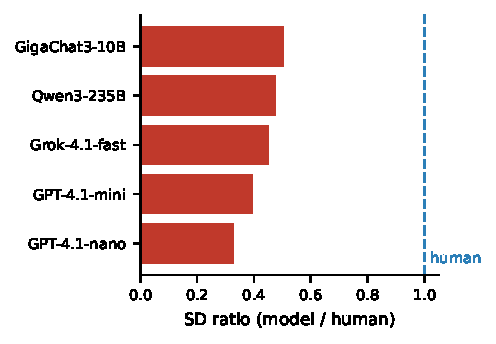
\includegraphics[width=0.85\linewidth]{figures/variance.pdf}
\caption{Response \emph{spread} relative to the humans being simulated, as a
ratio of standard deviations. Every model is substantially under-dispersed.}
\label{fig:variance}
\end{figure}

The style-only rung of the C2ST ladder, and what separability it carries,
is reported in Appendix~\ref{app:c2streading}.


% acl.sty already issues \bibliographystyle{acl_natbib}; repeating it here put a
% second \bibstyle into main.aux and made every bibtex run emit
% "Illegal, another \bibstyle command". Harmless in effect -- bibtex skips the
% duplicate and still builds the bibliography -- but it masks real bibtex errors
% behind a permanent one, so the redundant line is removed.
\bibliography{refs}

\end{document}
